\chapter{急性呼吸衰竭与急性呼吸窘迫综合征}

\section{前沿学术综述}

\subsubsection{历史发展}

急性呼吸窘迫综合征(ARDS)是急性呼吸衰竭最常见的类型。1967年Ashbaugh观察到12例重症患者(7例严重创伤、1例急性胰腺炎、1例病毒性肺炎、1例吉兰-巴雷综合征合并肺炎、2例药物中毒合并误吸),在原发病治疗过程中,均出现类似急性呼吸衰竭表现:呼吸频速、低氧血症、肺顺应性明显降低、肺泡表面张力明显升高。X线胸片早期为双肺斑片状浸润阴影,随病情进展,浸润阴影进一步扩大。最后9例患者死亡,其中7例尸检,发现肺重量明显增加,而且变硬,肺切面类似肝脏。光镜检查显示肺毛细血管充血、扩张,广泛肺泡萎陷,并有大量中性粒细胞浸润,肺泡内有透明膜形成。部分尸检标本有明显的间质纤维化。患者的低氧血症不能被吸氧等传统治疗手段纠正,但呼气末正压(PEEP)能够部分纠正低氧血症。鉴于上述患者有类似临床表现、病理结果和治疗反应,Ashbaugh将其归结为“成人呼吸窘迫综合征(亦为ARDS)”。4年后,“成人呼吸窘迫综合征”被正式推广采用。根据病因和病理特点不同,ARDS还被称为休克肺、灌注肺、湿肺、白肺、成人透明膜病变等。

近年来,许多学者认识到“成人呼吸窘迫综合征”这一名称并不合适。并非仅发生在成人,儿童亦可发生。ARDS的特点在于急性起病。因此,为澄清并统一概念,1992年欧美危重病及呼吸疾病专家召开了ARDS联席会议
\protect\hyperlink{text00011.htmlux5cux23ch1-10}{\textsuperscript{{[}1{]}}}
,将ARDS中的“A”由成人(adult)改为急性(acute),称为“急性呼吸窘迫综合征”。以往认为,ARDS是肺部遭受直接损伤的结果,目前认为各种原因导致机体失控的炎症反应才是ARDS的根本原因,急性肺损伤与ARDS是连续的病理生理过程,ARDS并不是孤立的疾病,而是多脏器功能障碍综合征(MODS)在肺部的表现。

\subsubsection{流行病学}

流行病学调查显示,ARDS是临床常见危重症。根据1994年欧美联席会议提出的ALI/ARDS诊断标准
\protect\hyperlink{text00011.htmlux5cux23ch1-10}{\textsuperscript{{[}1{]}}}
,ALI发病率为每年18/10万,ARDS为每年(13~23)/10万。2005年的研究显示,ALI/ARDS发病率分别在每年79/10万和59/10万
\protect\hyperlink{text00011.htmlux5cux23ch2-10}{\textsuperscript{{[}2{]}}}
,提示其发病率明显增高,甚至可与胸部肿瘤、AIDS、哮喘或心肌梗死等相提并论
\protect\hyperlink{text00011.htmlux5cux23ch3-10}{\textsuperscript{{[}3{]}}}
,显著增加了社会和经济负担。

虽然不同研究对ARDS病死率的报道差异较大,但总体来说,目前ARDS的病死率仍较高。自1994年达成ARDS诊断共识以来,ARDS总体病死率并无明显降低。对1994~2006年国际正式发表的ARDS临床研究进行荟萃分析,18900例ARDS患者的病死率为44.3%,与1967~1994年病死率(30%~50%)相比并无明显降低
\protect\hyperlink{text00011.htmlux5cux23ch4-10}{\textsuperscript{{[}4{]}}}
。中国上海市15家成人重症医学科2001年3月至2002年3月ARDS患者的病死率也高达68.5%
\protect\hyperlink{text00011.htmlux5cux23ch5-10}{\textsuperscript{{[}5{]}}}
。不同研究中,ARDS的病因构成、疾病状态和治疗条件的不同可能是导致其病死率不同的主要原因。

\subsubsection{治疗进展}

在治疗过程中不应把ARDS孤立对待,而应该将其视为多脏器功能障碍综合征的一部分。在呼吸支持治疗的同时,应特别重视对于原发病的治疗和其他脏器功能支持治疗。近年来,体外膜氧合技术的应用为进一步降低重症ARDS患者的病死率带来了新的希望。此外,针对ARDS肺损伤本质的干细胞治疗也受到越来越多的关注,可能为ALI/ARDS的治疗开辟新的途径,但目前仍处于动物实验阶段。

(1)原发病治疗 及时去除或控制致病因素是ARDS病因治疗的重要环节,根据ARDS的病因不同,主要包括充分引流感染灶、有效地清创和合理使用抗生素等。机体过度的炎症反应是导致ARDS的根本原因,调控机体的炎症反应是ARDS病因治疗的关键。虽然在动物实验中,应用单克隆抗体或拮抗剂可明显减轻肺损伤,但多数临床试验却获得阴性结果。目前,在调控机体炎症反应方面尚未取得突破性进展,但调控炎症反应仍然是降低ARDS患者病死率的希望。呼吸支持治疗从本质上来说,不可能从根本上改善ARDS患者的预后,因此,对调控机体炎症反应进行更深入研究非常必要。

(2)呼吸支持治疗 机械通气是ARDS呼吸支持治疗的主要方法,也是目前发展较为迅速的领域。近年来,基于对ARDS的病理生理和呼吸机相关性肺炎的新认识,一些新的通气策略逐步应用于ARDS的临床治疗,体外膜氧合技术的应用使保证气体交换的同时减缓肺损伤成为可能,为患者呼吸功能的修复赢得了时间。

肺保护性通气策略:由于ARDS患者大量肺泡塌陷,肺容积明显减少,常规或大潮气量通气易导致肺泡过度膨胀加重肺损伤,因此,为避免或减轻机械通气所致的肺损伤,主张对ARDS患者进行机械通气时应采用小潮气量(一般4~7ml/kg)通气,即肺保护性通气。近年来,人们逐步意识到小潮气量并非是避免肺损伤的关键因素,而气道平台压力能够客观反映肺泡内压,气道平台压力过度升高可导致呼吸机相关肺损伤。目前认为,ARDS肺保护性通气策略的关键是将气道平台压限制在30cm
H\textsubscript{2} O(1cm H\textsubscript{2} O=0.098kPa)以下。

肺开放策略:限制气道平台压往往不利于已塌陷的肺泡复张,采用肺保护性通气策略的同时,实施肺开放策略是非常必要,其核心是采用各种方法促进塌陷的肺泡复张,即“开放肺”,并应用最佳呼气末正压保持肺泡处于开放状态,即“维持肺开放”。促进肺复张的方法有多种,除了以往常用的叹息和控制性肺膨胀外,近年又提出了压力控制法和呼气末正压递增法等肺复张手法
\protect\hyperlink{text00011.htmlux5cux23ch6-10}{\textsuperscript{{[}6{]}}}
。此外,近年也有学者主张采用气道压力释放通气或高频振荡通气来实施肺开放。改变患者的体位,如俯卧位等,可改善患者胸腔内的压力梯度,也是促进肺复张的有效方法。

最佳呼气末正压的选择方法一直存在争议,以往有学者提出采用氧合法、最大氧输送法或依据肺静态压力-容积曲线低位转折点压力来选择呼气末正压。近年来,有学者提出了采用静态压力-容积曲线第三拐点压力,最大肺顺应性、肺牵张指数法及根据跨肺压等呼气末正压选择的新方法,但仍需大规模临床试验加以证实。

体外膜氧合治疗:体外膜氧合治疗适用于病因可逆且传统治疗无效的重症ARDS患者。重症ARDS患者进行体外膜氧合治疗的根本目的是在保障二氧化碳和氧交换的基础上,避免高潮气量和高气道压导致的肺损伤,为肺部病变的修复赢得时间。对于重症ARDS患者,可通过静脉静脉体外膜氧合或体外二氧化碳排出等方式改善气体交换,同时结合肺保护性的通气策略减缓肺损伤。自2009年体外膜氧合成功用于抢救H1N1流感导致的重症ARDS患者以来,全球体外膜氧合的关注度及治疗例数明显升高,2009年《柳叶刀》杂志发表英国CESAR研究报告,通过对180例ARDS患者的随机对照研究发现,体外膜氧合+传统治疗方法结合组生存率(63%)明显高于单纯传统治疗组(47%)
\protect\hyperlink{text00011.htmlux5cux23ch7-10}{\textsuperscript{{[}7{]}}}
。我国体外膜氧合治疗重症ARDS尚处于起步阶段,如何统筹并规范地开展体外膜氧合治疗仍需要进一步探讨。

体外膜氧合是在机械通气维持氧合的效果差、呼吸功能在短期内又无法纠正的情况下,可应用体外膜氧合进行呼吸支持,有助于降低呼吸机条件,减轻呼吸机相关肺损伤,并为患者呼吸功能恢复争取时间。

(3)肺外器官功能支持治疗 肺外器官的功能支持和全身营养支持是ARDS治疗不可忽视的重要环节。以往由于呼吸支持手段不足,ARDS患者往往死于顽固的低氧血症,近年来,早期有力的呼吸支持使患者不再死于低氧血症,主要的病死原因是继发的多脏器功能衰竭。ARDS的恶化可能诱发或加重其他器官发生功能障碍,而肺外器官的衰竭反过来又可加重ARDS。因此,加强肺外器官功能支持,防止多脏器功能衰竭的发生、发展可能是当前改善ARDS患者预后的重要手段。在保证脏器充分灌注的基础上实施限制性液体管理策略减轻脏器水肿是非常必要的。早期营养支持也值得重视,尽早开始肠内营养,有助于恢复肠道功能和保持肠黏膜屏障功能,防止细菌及毒素移位引起多脏器功能衰竭。此外,循环功能、肾功能、肝功能等器官功能的支持也不可忽视。总之,在呼吸支持治疗的同时,应尽量避免损害并保护其他器官,只有这样,才有望最终改善ARDS患者的预后。

(4)细胞修复治疗 ALI/ARDS的主要病理改变为肺泡上皮细胞和毛细血管内皮细胞受损,促进损伤肺有效修复可能是ALI/ARDS治疗的关键所在。干细胞通过直接修复及其旁分泌作用可促进肺损伤的修复。此外,干细胞还可以作为基因治疗的载体,使得保护性基因在肺组织选择性和持久的表达,针对损伤局部提供治疗蛋白。虽然目前干细胞治疗的研究还处于动物实验阶段,但针对疾病本质的干细胞治疗,为ALI/ARDS的治疗提供了新的思路和希望。

\subsubsection{问题与前景}

目前认为,全身炎症反应是导致ARDS的共同途径,但一系列针对炎症反应调控的治疗(如糖皮质激素和细胞因子抗体或拮抗剂等)尚未取得满意效果,治疗上的进展多局限于呼吸或其他脏器功能的支持治疗,真正针对病因的治疗手段还很贫乏,难以从根本上解决ARDS的治疗问题。但这并不意味着其前景渺茫。近期体外膜氧合治疗广泛开展,在保证重症ARDS患者气体交换的同时,为肺损伤的修复赢得时间,已经在一定程度上减低了ARDS患者的病死率。干细胞治疗技术针对ARDS肺损伤的修复正逐步趋于成熟,为ARDS的治疗带来了新的希望。此外,ARDS发病的异质性也越来越引起人们的关注,目前研究显示,肺表面活性蛋白基因
\protect\hyperlink{text00011.htmlux5cux23ch8-10}{\textsuperscript{{[}8{]}}}
\textsuperscript{,}
\protect\hyperlink{text00011.htmlux5cux23ch9-10}{\textsuperscript{{[}9{]}}}
、血管紧张素转换酶基因
\protect\hyperlink{text00011.htmlux5cux23ch10-10}{\textsuperscript{{[}10{]}}}
\textsuperscript{,}
\protect\hyperlink{text00011.htmlux5cux23ch11-10}{\textsuperscript{{[}11{]}}}
、肿瘤坏死因子基因
\protect\hyperlink{text00011.htmlux5cux23ch12-10}{\textsuperscript{{[}12{]}}}
及白细胞介素-6
\protect\hyperlink{text00011.htmlux5cux23ch13-10}{\textsuperscript{{[}13{]}}}
等基因的差异可能与ARDS的易感性和预后相关。相信随着人们对ARDS发病机制更深入的了解,遗传学与分子生物学领域的研究也会在未来的治疗中发挥重要作用。

\section{临床问题}

\subsection{急性呼吸衰竭}

\subsubsection{何谓呼吸衰竭?如何诊断?}

呼吸衰竭(respiratory
failure)指外呼吸功能严重障碍导致的动脉血氧分压(PaO\textsubscript{2}
)降低或伴有动脉血二氧化碳分压(PaCO\textsubscript{2}
)增高的病理过程。呼吸衰竭按发病急缓分为急性呼吸衰竭和慢性呼吸衰竭,急性呼吸衰竭系指没有基础呼吸系统疾病的患者在短时间内发生的呼吸衰竭;慢性呼吸衰竭则指慢性呼吸系统疾病患者经过较长时间发展成的呼吸衰竭。慢性呼吸衰竭的患者由于各种诱因导致病情在短时间内急性加重者称为慢性呼吸衰竭急性加重(acute-on-chronic),其病理生理学改变和临床情况兼有急性呼吸衰竭的特点,临床上的处理措施也与急性呼吸衰竭相似。

低氧血症和高碳酸血症的临床表现并不特异,呼吸衰竭往往须进行血气分析方可确诊。诊断呼吸衰竭的主要血气标准是在海平面、标准大气压下,静息和吸空气时动脉血氧分压低于60mmHg(1mmHg=0.133kPa),伴或不伴有动脉血二氧化碳分压高于50mmHg。正常人动脉血氧分压随年龄、运动及所处的海拔高度而异,成年人在海平面静息时动脉血氧分压的正常范围为(13.3-0.043×年龄)±0.066kPa。动脉血二氧化碳分压极少受年龄影响,正常范围为40±5mmHg。当吸入气的氧浓度(FiO\textsubscript{2}
)增加时,可将氧合指数(respiratory failure
index,RFI)作为诊断呼吸衰竭的指标,RFI=动脉血氧分压/FiO\textsubscript{2}
,如≤300可诊断为呼吸衰竭。

\subsubsection{呼吸衰竭可分为哪些类型?}

呼吸衰竭必定有动脉血氧分压的降低。根据动脉血二氧化碳分压是否升高,可将其分为低氧血症型(Ⅰ型)和伴有低氧血症的高碳酸血症型(Ⅱ型)呼吸衰竭。根据主要发病机制不同,可分为通气性和换气性呼吸功能衰竭。根据病因的不同,可分为肺衰竭和泵衰竭。根据原发病变部位不同,可分为中枢性和外周性呼吸衰竭。根据发病的缓急,可分为慢性和急性呼吸衰竭。

\subsubsection{急性呼吸衰竭的常见病因有哪些?}

肺气体交换涉及两个环节,首先为通气(依赖“通气泵”作用),其次为肺换气(肺泡和血液之间的气体交换过程)。根据气体交换的两个环节,急性呼吸衰竭可分为肺衰竭和泵衰竭。

(1)引起肺衰竭的常见病因 肺衰竭是各种原因引起的肺泡气体交换不足的病理状态,主要表现为动脉血氧合不足,而无明显的二氧化碳潴留。动脉血二氧化碳可通过增加通气泵做功而排出。引起肺衰竭的主要病因包括:①呼吸道气流受限,包括喉头水肿、喉痉挛、异物、肿瘤、外伤、感染等上呼吸道梗阻,以及支气管哮喘严重发作、慢性支气管炎、阻塞性肺气肿和肺心病等广泛和严重的下呼吸道阻力增加;②肺实质疾病,主要包括严重肺部感染、毛细支气管炎、间质性肺疾病、肺水肿、肺栓塞和各种原因引起的肺实质损伤及急性呼吸窘迫综合征(ARDS)等。肺衰竭均伴有呼吸功增加,可导致呼吸肌疲劳,进一步恶化可引起泵衰竭。

(2)引起泵衰竭的常见病因 通气泵由胸廓、呼吸肌以及调节呼吸肌收缩和舒张的神经系统组成,其主要功能是保持一定的跨肺压梯度。引起泵衰竭常见病因包括------①呼吸肌疲劳或衰竭:气道阻力增加和肺顺应性降低导致呼吸肌过负荷;②胸廓和胸膜病变:严重气胸、大量胸腔积液、连枷胸、脊柱侧后凸、血胸、上腹部和胸部术后;③神经肌接头病变:重症肌无力、药物阻滞作用;④运动神经病变:脊髓损伤、脊髓灰质炎、吉兰-巴雷综合征、肌萎缩侧索硬化;⑤中枢神经系统抑制或功能紊乱:脑血管意外、病毒性脑炎、细菌性脑膜炎、药物中毒、脑水肿、颅脑外伤、中枢性通气不足综合征等。

\subsubsection{肺通气功能障碍的机制是什么?有何临床意义?}

外呼吸包括肺通气和肺换气,前者指肺泡与外界气体交换的过程,后者指肺泡气与血液之间的气体交换过程。呼吸衰竭是肺通气和(或)肺换气功能障碍的结果。

肺通气不足导致肺泡通气量不足会使肺泡气氧分压下降和肺泡气二氧化碳分压升高,因而流经肺泡毛细血管的血液不能被充分动脉化,导致动脉血氧分压下降和动脉血二氧化碳分压增高,最终出现Ⅱ型呼吸衰竭。此时,动脉血二氧化碳分压的增值与动脉血氧分压降值成一定比例关系,其比值相当于呼吸商(R)。P\textsubscript{A}
O\textsubscript{2} =PiO\textsubscript{2} -P\textsubscript{A}
CO\textsubscript{2} /R,其中PiO\textsubscript{2}
为吸入气氧分压,在海平面吸空气时大约为150mmHg。当肺泡通气量减少一半时,肺泡气二氧化碳分压由正常40mmHg增加至80mmHg,在R为0.8时,肺泡气氧分压就由正常的100mmHg降低至50mmHg,两变化值之商为0.8,等于呼吸商,这是单纯肺低通气时血气变化的特点。

肺泡气二氧化碳分压与动脉血二氧化碳分压无明显差异,动脉血二氧化碳分压是反映总肺泡通气量变化的最佳指标。但动脉血二氧化碳分压与总肺泡通气量之间的关系并非为线性。相同肺泡通气量变化值,在通气不足或通气过度时对动脉血二氧化碳分压的影响比较显著。肺泡通气量低于正常时,肺泡气氧分压随通气量增加而升高,但当通气量高于4L/分钟以上时,肺泡气氧分压增加趋势变缓。在轻度通气不足时,动脉血氧饱和度仍较高;但严重通气不足时动脉血氧饱和度显著降低。

肺通气功能障碍包括限制性和阻塞性通气不足。

限制性通气不足是指吸气时肺泡的扩张受限引起的肺泡通气不足。其原因有:①呼吸肌活动障碍,包括中枢或周围神经的器质性病变如脑外伤、脑血管意外、脊髓灰质炎等;由于镇静、安眠和麻醉剂过量引起的呼吸中枢抑制;呼吸肌本身的收缩功能障碍如呼吸肌疲劳及呼吸肌萎缩;由低钾、缺氧和酸中毒等导致的呼吸肌无力等;②胸廓顺应性降低,如严重胸廓畸形、胸膜纤维化等;③肺顺应性降低,如严重肺纤维化或肺泡表面活性物质减少可使肺顺应性降低;④大量的胸腔积液或张力性气胸使肺扩张受限。

阻塞性通气不足指气道狭窄或阻塞所致的通气障碍。影响气道阻力最主要的因素是气道内径。气管痉挛、管壁肿胀或纤维化,管腔被黏液、渗出物、异物等阻塞,肺组织弹性降低以致对气道管壁的牵引力减弱等,均可使气道内径变窄或不规则而增加气流阻力,从而引起阻塞性通气不足。气道阻塞可分为中央性与外周性,中央性气道阻塞指气管分叉处以上的气道阻塞,若阻塞位于胸外,吸气时气体流经病灶引起压力降低,可使气道内压明显低于大气压,导致气道狭窄加重,而呼气时则相反,故患者表现为明显吸气性困难;如阻塞位于胸内,呼气时胸腔内压升高而压迫气道,使气道狭窄加重,而吸气时则相反,故患者表现为呼气性呼吸困难。外周性气道阻塞多见于慢性阻塞性肺疾病时,主要表现为呼气性呼吸困难。

\subsubsection{何谓肺通气/血流比例失调?有何临床意义?}

肺通气/血流比例失调是肺换气功能障碍的一种形式。肺内气体交换有赖于单位时间内肺泡通气量和肺泡血流灌注量之间一定的比例。正常情况下肺通气/血流之比为0.8。当病变引起局部肺通气发生变化而血流未相应变化,或局部血流变化而通气未相应变化时,即发生肺通气/血流比例失调。即使在健康人体,肺各部分肺通气/血流比例也并非均匀分布,直立位时,由于重力作用血流量自肺尖到肺底逐步递增,而胸腔内负压上部比下部大,故肺尖部的肺泡扩张程度较大,从而使肺通气/血流比例自上而下递减。

肺通气/血流比例失调是呼吸衰竭最常见和最重要的机制。急性呼吸窘迫综合征(ARDS)患者严重的低氧血症主要与肺通气/血流比例失调有关。病理状态下,肺通气/血流比例失调常见的原因如下。

(1)部分肺泡通气不足 慢性阻塞性肺疾病、哮喘、肺水肿、肺纤维化等往往引起肺泡通气严重不均匀。病变部分通气明显减少,而血流未相应减少,使肺通气/血流比例显著降低,以致流经这部分肺泡的静脉血未能充分动脉化便掺入动脉血内,故称静脉血掺杂,又称功能性分流。此时动脉血氧分压往往降低,如代偿性通气足够强,尚可使动脉血二氧化碳分压正常或降低,如代偿不足,使总肺泡通气量低于正常,则动脉血二氧化碳分压高于正常。

(2)部分肺泡血流不足 肺动脉栓塞、弥散性血管内凝血、肺血管痉挛等,都可使肺部分血流减少或中断,肺通气/血流比例可显著高于正常或为无穷大,肺泡通气不能被充分利用,称为死腔样通气。此时,流经病变区血液的动脉血氧分压显著升高,但其动脉血氧含量却增加很少,健康肺区却因血流量明显增加而使这部分血液不能充分动脉化,其动脉血氧分压和动脉血氧含量均显著降低。最终混合而成的动脉血之动脉血氧分压降低,动脉血二氧化碳分压的变化则取决于代偿性呼吸增强的程度,可以降低、正常或升高。

(3)真性分流 正常情况下,一部分静脉血经支气管静脉和极少的肺动-静脉交通支直接流入肺静脉,即为解剖分流。由于这部分血液完全未经气体交换过程,故属于真性分流。病变导致肺动静脉短路开放,真性分流增加。此外,在肺实变和肺不张时,病变肺完全失去通气功能,但仍有血流,肺通气/血流比例为0,也属于真性分流。由真性分流导致的呼吸衰竭的特征是动脉血氧分压降低,且吸入高浓度氧动脉血氧分压不能提高,而功能性分流时吸入高浓度氧动脉血氧分压往往可提高,用这种方法可对二者进行鉴别。

\subsubsection{弥散障碍的机制是什么?对动脉血气有何影响?}

弥散障碍是肺换气功能障碍的一种形式,指肺泡膜面积减少或肺泡膜异常增厚和弥散时间缩短而引起的气体交换障碍。常见的原因包括:①肺泡膜面积减少。正常成人肺泡总面积约为80m\textsuperscript{2}
,面积减少一半以上时,才会发生换气功能障碍。肺泡膜面积减少常见于肺实变、肺不张和肺叶切除等;②肺泡膜厚度增加。肺泡膜的薄部为气体交换的部位,它是由肺泡上皮、毛细血管内皮及两者共有的基底膜所构成,其厚度不到1μm,是气体交换的部位。虽然气体从肺泡腔到达红细胞内还需经过肺泡表面的液体层、血管内血浆和红细胞膜,但正常情况下总厚度不到5μm,故正常气体交换很快。当肺水肿、肺泡透明膜形成、肺纤维化及肺泡-毛细血管扩张或稀血症导致血浆层变厚时,可因弥散距离增宽而使弥散速度减慢。

单纯肺泡膜病变患者在静息时一般不出现血气异常。因为正常静息时,血液流经肺泡-毛细血管的时间约为0.75秒,而血液氧分压只需0.25秒就可升至肺泡气氧分压水平。肺泡膜病变时,虽然弥散速度减慢,但在静息时气体交换在0.75秒内仍可达到血气与肺泡气的平衡而不发生血气异常。在体力负荷增加等使心输出量增加和肺血流加快时,血液和肺泡接触时间过于缩短,导致低氧血症。但肺泡膜病变加上肺血流增快一般不会引起动脉血二氧化碳分压增高。因为二氧化碳在水中的溶解度比氧气大,弥散速度比氧快,能较快地弥散入肺泡,故只要患者肺泡通气量正常,就可保持动脉血二氧化碳分压正常。

\subsubsection{低氧血症和缺氧有何不同?}

低氧血症(hypoxemia)和缺氧(hypoxia)是两个不同的概念,不能等同视之。低氧血症是指血氧含量降低,而缺氧是指因氧供减少、氧耗增加或利用氧障碍引起细胞发生代谢、功能和形态结构异常变化的病理过程。缺氧又根据其原因不同分为4种类型。

(1)低张性缺氧 是以动脉血氧分压降低为基本特征的缺氧。低张性缺氧时,动脉血氧分压降低,与血红蛋白结合的氧量减少,造成动脉血氧含量降低。

(2)血液性缺氧 是由于血红蛋白质或量的改变,以致血液携带氧的能力降低而引起的缺氧。血液性缺氧时,动脉血氧分压及SaO\textsubscript{2}
正常,但因血红蛋白质或量的改变,造成动脉血氧含量的降低。

(3)循环性缺氧 是指因组织血流量减少引起的组织氧供不足。由于缺氧是由组织灌注减少引起的,动脉血氧分压和氧含量正常,因此,循环性缺氧不能归于低氧血症的范畴。

(4)组织性缺氧 是指在组织氧供正常的情况下,因细胞不能有效利用氧而导致的缺氧。由于缺氧的原因是组织利用氧障碍,动脉血氧分压和氧含量正常,因此,组织性缺氧也不能归于低氧血症的范畴。

总之,缺氧是比低氧血症范畴更广的概念,将缺氧简单的理解为低氧血症是不全面的。

\subsection{急性呼吸窘迫综合征}

\subsubsection{何谓急性呼吸窘迫综合征?}

急性呼吸窘迫综合征(ARDS)是发生于严重感染、休克、创伤及烧伤等疾病过程中,由于肺毛细血管内皮细胞和肺泡上皮细胞损伤引起弥漫性肺间质及肺泡水肿,以进行性低氧血症、呼吸窘迫为特征的临床综合征。X线胸片呈现斑片状阴影为其影像学特征;肺容积减少、肺顺应性降低和严重的通气/血流比例失调为其病理生理特征。

\subsubsection{急性呼吸窘迫综合征的常见病因和危险因素有哪些?有何临床意义?}

多种病因均可导致急性呼吸窘迫综合征(ARDS)。根据肺损伤的机制,可将ARDS的病因分为直接肺损伤因素和间接肺损伤因素。

直接肺损伤因素主要包括:①严重肺部感染,包括细菌、真菌、病毒及肺囊虫感染等;②误吸,包括胃内容物、烟雾及毒气等误吸;③肺挫伤;④淹溺;⑤肺栓塞,包括脂肪、羊水、血栓栓塞等;⑥放射性肺损伤;⑦氧中毒等。

间接肺损伤因素主要包括:①严重感染及感染性休克;②严重非肺部创伤;③急性重症胰腺炎;④体外循环;⑤大量输血;⑥大面积烧伤;⑦弥散性血管内凝血;⑧神经源性(见于脑干或下丘脑)损伤等。

病因不同ARDS的患病率也明显不同,严重感染时ARDS患病率可高达25%~50%,大量输血可达40%,多发性创伤时达到11%~25%,严重误吸ARDS患病率也可达9%~26%。同时存在两或三个发病危险因素时,ARDS患病率进一步升高。另外,暴露于危险因素的时间越久,ARDS的患病率越高,危险因素持续24、48及72小时时,ARDS患病率分别为76%、85%和93%。目前认为,各种致病因素导致的全身炎症反应是ARDS的根本原因。在ARDS的防治过程中,积极控制原发病,遏制其诱导的全身失控性炎症反应,是预防和治疗ARDS的必要措施。

\subsubsection{急性呼吸窘迫综合征主要有哪些病理生理特征?}

急性呼吸窘迫综合征(ARDS)的基本病理生理改变,是肺泡上皮和肺毛细血管内皮通透性增加所致弥漫性肺间质及肺泡水肿。由于肺泡及间质水肿、肺泡表面活性物质减少及肺泡塌陷导致的肺容积减少、肺顺应性降低和严重的通气/血流(V/Q)比例失调,特别是肺内分流明显增加,是ARDS的病理生理特征。

(1)肺容积减少 ARDS患者早期就存在肺容积减少,表现为肺总量、肺活量、潮气量和功能残气量明显低于正常。由于ARDS患者的肺容积明显减少,实际参与通气的肺泡减少,常规或大潮气量机械通气易导致肺泡过度膨胀和气道平台压力过高,加重肺及肺外器官的损伤。

(2)肺顺应性降低 肺顺应性降低是ARDS的特征之一,表现为需要较高的气道压力,才能达到所需的潮气量。肺顺应性降低主要与肺泡表面活性物质减少引起的表面张力增高和肺不张、肺水肿导致的肺容积减少有关。ARDS亚急性期,肺组织如出现广泛的纤维化,可使肺顺应性进一步降低。

(3)肺通气/血流比例失调 肺通气/血流比例失调是导致ARDS患者严重低氧血症的主要原因。间质性肺水肿压迫小气道,表面活性物质减少导致肺泡部分萎陷,均可引起相应肺单位通气不足,导致肺通气/血流比例降低,即功能性分流
\protect\hyperlink{text00011.htmlux5cux23ch8-10}{\textsuperscript{{[}8{]}}}
,而广泛的肺不张和肺泡水肿引起局部肺单位只有血流而无通气,即真性分流,是导致顽固低氧血症的主要原因。研究显示,ARDS早期的肺内分流率可高达30%以上。ARDS机械通气时应用肺复张手法及一定水平的呼气末正压(PEEP),可使部分肺泡通气增加,减少肺内分流,进而改善氧合。ARDS时,肺微血管痉挛或狭窄、肺栓塞及血栓形成可使部分肺单位周围毛细血管血流量明显减少或中断,肺通气/血流比例升高,即导致死腔样通气。ARDS后期死腔率可高达60%。

\subsubsection{急性呼吸窘迫综合征的主要病理生理过程是什么?}

大量的临床活检和尸检资料表明,急性呼吸窘迫综合征(ARDS)病理形态学改变大致分为3个阶段。

(1)渗出期(exudative
phase) 发病后24~96小时。该期的主要特点是肺水肿、出血和充血性肺不张,肺血管内有中性粒细胞扣留和微血栓形成,有时可见脂肪栓子,肺间质内中性粒细胞浸润。电镜下,可见肺泡表面活性物质层出现断裂、聚集或脱落到肺泡腔。Ⅰ型上皮细胞发生变性,其薄区出现坏死;Ⅱ型上皮细胞空泡化,板层小体减少或消失。在上皮细胞破坏明显处有透明膜形成,透明膜由坏死细胞碎片、纤维蛋白以及血浆渗出物组成,在呼吸性细支气管和肺泡管处尤为明显。

(2)增生期(proliferative
phase) 发病后3~7天。此期主要表现为Ⅱ型上皮细胞大量增生,在某些部位几乎覆盖整个肺泡表面,肺水肿减轻,肺泡膜因Ⅱ型上皮细胞增生、间质中性粒细胞和成纤维母细胞浸润而增厚,毛细血管数目减少。

(3)纤维化期(fibrotic
phase) 发病后7~10天。肺泡间隔内纤维组织增生显著,透明膜可弥漫分布于全肺,此后透明膜中纤维母细胞浸润,逐渐转化为纤维组织。肺泡管的纤维化是晚期ARDS患者的典型病理变化。

总的来说,肺实质细胞损伤是ARDS的主要病理特点。早期ARDS或急性肺损伤是以肺毛细血管内皮细胞损伤和功能障碍导致水和蛋白向间质渗出增加为特点,而肺毛细血管内皮细胞损伤后进一步损伤肺泡上皮细胞,使肺泡内水增加,肺泡塌陷,导致肺不张。由于ARDS发病急、进展快,多数患者在渗出期或增生期死亡,肺的纤维化是ARDS最严重的后遗症。ARDS的病理过程具有不均一性的特点,即在不同区域的肺组织可能处于不同的病理阶段,因此,临床上往往很难就肺部病变的整体进行具体的病理阶段区分。

\subsubsection{如何评价机体炎症反应在急性呼吸窘迫综合征发病中的地位?}

过去认为急性呼吸窘迫综合征(ARDS)是感染或组织损伤对肺直接打击的结果。目前认为,感染、创伤后的全身炎症反应失控是导致ARDS的根本原因。大量研究显示:①细菌、内毒素或损伤刺激后,机体异常释放大量炎症介质;②给动物注射炎症介质,能复制ARDS模型;③注射炎症介质单克隆抗体,可防止动物发生ARDS。这些证据似乎已阐明了ARDS的发病机制,但研究显示,单纯应用某种炎症介质的单克隆抗体往往并不能取得良好的疗效。感染或创伤导致ARDS等器官功能损害的过程表现为两种极端:一是大量炎症介质瀑布样释放,而内源性抗炎介质又不足以抵消其作用,结果导致全身炎症反应综合征;另一个是内源性抗炎介质释放过多,结果导致代偿性抗炎反应综合征。全身炎症反应综合征和代偿性抗炎反应综合征失衡的后果是炎症反应的扩散和失控,不但损伤局部组织细胞,同时打击远隔的器官,导致肺功能损伤。因此,就本质而言,ARDS是全身炎症反应综合征和代偿性抗炎反应综合征失衡的结果,也就是机体炎症反应失控的结果。在ARDS的防治过程中,积极控制原发病,遏制其诱导的全身失控性炎症反应,是预防和治疗ARDS的必要措施。

\subsubsection{急性呼吸窘迫综合征的诊断标准是什么?}

自从1967年急性呼吸窘迫综合征(ARDS)概念提出以来,曾制定过多个诊断标准,但均未被广泛采用。1988年Murray等提出了ARDS的评分法诊断标准,对ARDS做量化诊断。该标准需满足3个条件:①急性起病;②致病因素明确;③达到一定程度的肺损伤(轻、中、重度损伤)。其中肺损伤程度由氧合指数、呼气末正压水平、X线胸片中受累象限数及肺顺应性变化评分决定。评分>2.5分为重度肺损伤,即ARDS;评分0.1~2.5为轻中度肺损伤。该标准强调了肺损伤从轻到重的连续发展过程,对肺损伤做了量化评价。

Murray等提出的标准尽管有利于科研,但应用过于繁琐,难以在临床上推广。目前临床上广泛采用1994年欧美联席会议提出的ARDS诊断标准------ARDS需满足:①急性起病;②氧合指数≤200mmHg(不管呼气末正压水平);③正位X线胸片显示双肺均有斑片状阴影;④肺动脉嵌顿压≤18mmHg,或无左心房压力增高的临床证据。如氧合指数≤300mmHg且满足上述其他标准则诊断为急性肺损伤(ALI),反映了ARDS是ALI的严重阶段,二者是连续的病理生理过程。该标准与以往标准的主要区别是:①呼气末正压的氧合改善效应具有时间依赖性,且呼气末正压水平的提高与氧合改善并非正相关,故诊断时不再考虑呼气末正压水平;②机械通气受医师的经验等多种因素影响,故也未把机械通气作为诊断ARDS的条件;③将肺动脉嵌顿压≤18mmHg或无左心房压力增高的临床证据列入诊断条件,有利于排除心源性肺水肿;④反映了ARDS和ALI是连续的病理生理过程,有利于早期诊断和治疗。欧美联席会议的ARDS诊断标准较易实施,对临床价值更大,目前已被广泛采用。

虽然欧美联席会议的ARDS诊断标准广泛应用于临床,但研究显示其准确性不高,存在诸多需要改进之处。2011年10月在德国柏林举行的第23届欧洲危重病医学年会上,ARDS标准再次被推陈出新,形成柏林标准
\protect\hyperlink{text00011.htmlux5cux23ch14-10}{\textsuperscript{{[}14{]}}}
,该标准基于当前流行病学证据、生理学概念以及相关临床研究结果,由欧美等国重症医学专家协商制定,主要从起病时间、低氧血症程度、肺水肿来源、X线胸片及其他生理学紊乱5个方面进行描述(表\ref{tab5-1})。该标准是对之前各个标准的总结,相对较为全面。Gattinoni等对柏林标准进行了验证,发现其能有效区别出ARDS的严重程度,并且有助于较为准确地判断预后。但是这样的结论仍需要后续的临床研究予以验证。

\begin{table}[htbp]
{\centering
\caption{ARDS柏林诊断标准}
\label{tab5-1}
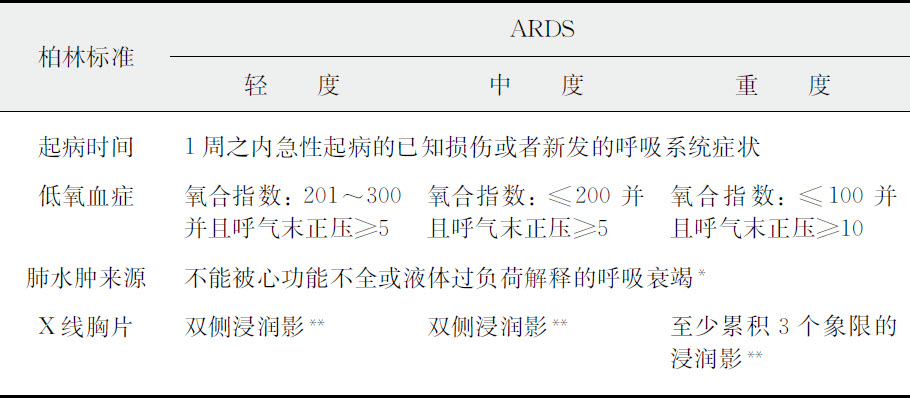
\includegraphics{./images/Image00046.jpg}}

\footnotesize
* 如果没有危险因素,需要客观指标的评估;

**
通过专业影像学培训后阅读胸片,浸润影不能被胸腔积液、结节、肿块、肺叶塌陷所完全解释。
\end{table}



\subsubsection{如何对急性呼吸窘迫综合征的肺损伤程度进行定量评价?}

对肺损伤程度的临床评价,主要有以下指标。

(1)1988年Murray等提出的肺损伤程度评分法 此方法对急性呼吸窘迫综合征(ARDS)的肺损伤程度做量化分析。Murray急性肺损伤评分包括3方面内容(表\ref{tab5-2}):①肺损伤程度的定量评分;②具有ARDS患病的危险因素;③合并肺外器官功能不全。根据氧和指数、呼气末正压水平、X线胸片中受累象限数及肺顺应性变化的评分评价肺损伤程度。评分>2.5分为重度肺损伤,即ARDS;0.1~2.5分者为轻中度肺损伤。该标准强调了肺损伤从轻到重的连续发展过程,对肺损伤做量化评价。Owens等研究显示肺损伤评分与肺脏受累范围呈显著正相关(\emph{r}
=0.75,\emph{P} <0.01),而且也与肺血管通透性密切相关(\emph{r}
=0.73,\emph{P}
<0.01)。可见,该标准可较准确地评价肺损伤程度,目前在临床中应用最为广泛。

\begin{table}[htbp]
{\centering
\caption{Murray肺损伤评分\textsuperscript{*}}
\label{tab5-2}
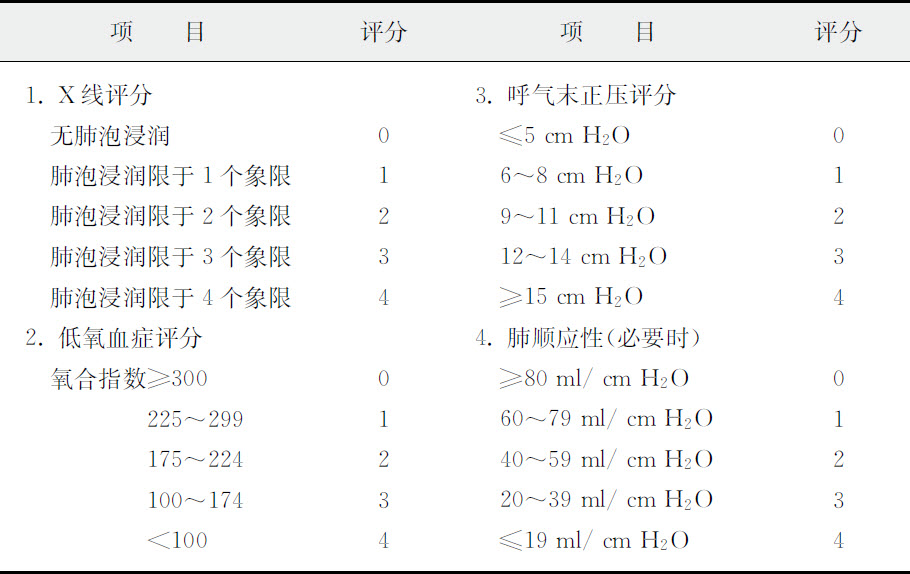
\includegraphics{./images/Image00047.jpg}}

\footnotesize *
上述4项或3项(除肺顺应性)评分的总和除以项目数(分别为4或3),就得到肺损伤评分结果。
\end{table}



(2)气体交换障碍的程度 氧合指数可反映ARDS早期肺损伤程度,部分研究认为该指标与ARDS患者的预后具有相关性。

(3)急性生理和既往健康状况评分(APACHE)Ⅱ和ⅢAPACHE评分系统并非是专门为ARDS患者设计的,但其对ARDS患者的预后有一定预测价值。

\subsubsection{急性呼吸窘迫综合征如何进行临床分期?有何意义?}

目前对于急性呼吸窘迫综合征(ARDS)的临床分期仍沿用1968年Bone提出的创伤后ARDS分期方法------①创伤早期:创伤或感染后数天内,往往表现为呼吸偏快,轻度鼻翼扇动,动脉血二氧化碳分压降低,但动脉血氧分压多正常;②相对稳定期:持续1~3天,该期患者呼吸逐渐平稳,X线胸片正常;③急性呼吸衰竭期:出现于创伤感染后1周左右,呼吸窘迫明显、呼吸频速、紫绀,动脉血氧分压明显降低,二氧化碳分压亦下降,X线胸片有非对称斑片状阴影;④终末期:表现为严重呼吸窘迫和紫绀,动脉血氧分压明显降低,二氧化碳分压明显升高,X线胸片有较多斑片状阴影,往往引起其他器官的功能损害或衰竭。

虽然部分ARDS患者病情进展迅速,临床分期表现并不明显,但ARDS的临床分期仍有助于ARDS的早期诊断和早期预防。首先,严重创伤、感染、手术或休克等本身是急性肺损伤的高危因素,应高度警惕可能发生ARDS;其次,患者在创伤或手术后可能出现短暂的稳定期,临床医生不应被患者暂时的稳定所迷惑,应采取积极措施,防止ARDS发生;第三,ARDS的临床诊断不应硬搬诊断标准,对于有危险因素和早期临床表现的患者,即使不符合ARDS诊断标准,也应该按ARDS处理。

\subsubsection{急性呼吸窘迫综合征与心源性肺水肿或心衰在临床上如何鉴别?}

急性呼吸窘迫综合征(ARDS)与心源性肺水肿的临床表现有很多相似之处,但临床治疗手段相差甚远,如不能及时鉴别,往往会延误病情,导致严重后果。

ARDS与心源性肺水肿的不同临床特点见表\ref{tab5-3}。

\begin{table}[htbp]
\centering
\caption{ARDS与心源性肺水肿的鉴别诊断}
\label{tab5-3}
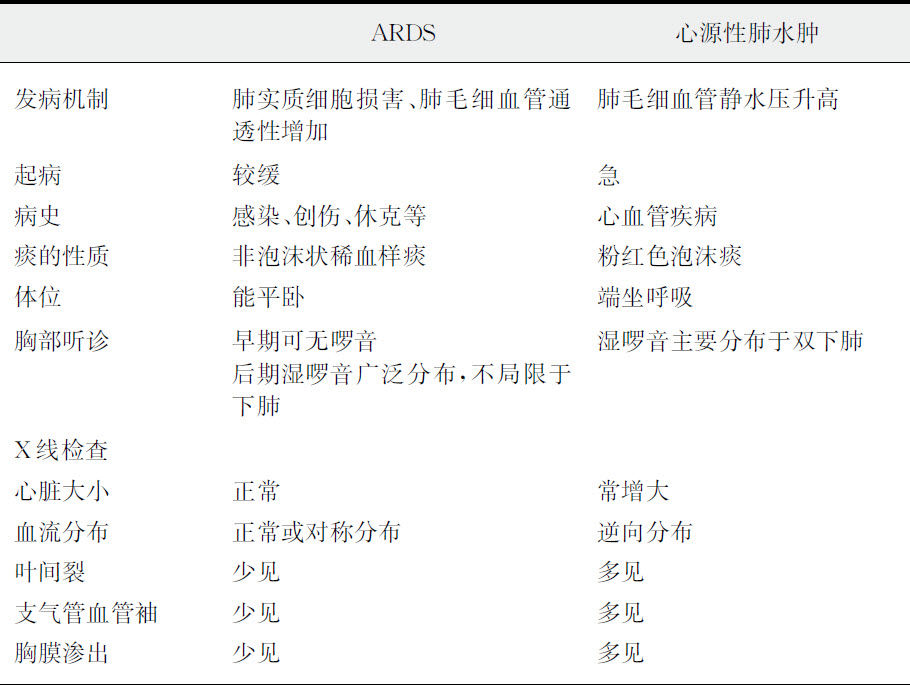
\includegraphics{./images/Image00048.jpg}
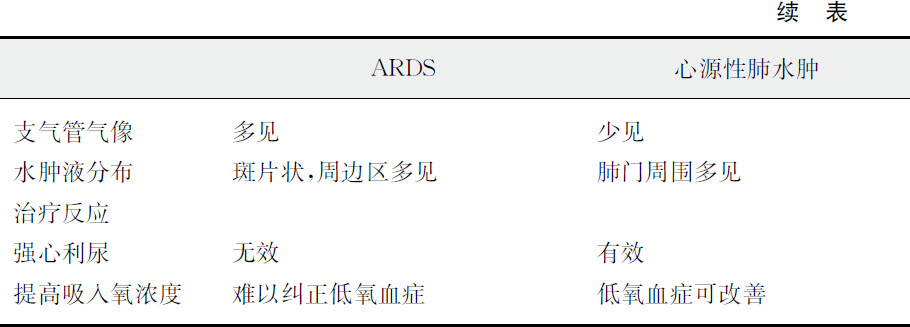
\includegraphics{./images/Image00049.jpg}
\end{table}



\subsection{急性呼吸窘迫综合征的病因与呼吸支持治疗}

\subsubsection{急性呼吸窘迫综合征有哪些病因治疗手段?}

(1)控制致病因素 及时去除或控制致病因素是急性呼吸窘迫综合征(ARDS)病因治疗的重要环节,主要包括充分引流感染灶、有效清创和合理使用抗生素。当然,腹腔或肺部等处感染的蔓延、急性胰腺炎的发展都会使病因治疗相当困难。

(2)调控机体的炎症反应 调控机体的炎症反应是ARDS病因治疗的关键。机体过度的炎症反应是导致ARDS的根本原因,调控机体的炎症反应不但是ARDS病因治疗的重要手段,也可能是控制ARDS、降低病死率的关键。虽然在动物实验中,应用单克隆抗体或拮抗剂中和肿瘤坏死因子、白介素-1和白介素-8等细胞因子可明显减轻肺损伤,但多数临床试验获得阴性结果。两项大样本临床试验观察了抗肿瘤坏死因子单克隆抗体(Afelimomab)治疗严重感染的临床疗效,尤其是对于白介素-6水平升高患者的疗效,结果也不一致。其中MONARCS研究(\emph{n}
=2634)显示,无论在白介素-6高水平还是低水平的严重感染患者,Afelimomab治疗组的病死率明显降低
\protect\hyperlink{text00011.htmlux5cux23ch2-10}{\textsuperscript{{[}2{]}}}
。但另一项研究并不降低病死率
\protect\hyperlink{text00011.htmlux5cux23ch1-10}{\textsuperscript{{[}1{]}}}
。细胞因子单克隆抗体或拮抗剂是否能够用于ARDS的治疗,目前尚缺乏临床研究证据。此外,糖皮质激素、布洛芬等环氧化酶抑制剂、N-乙酰半胱氨酸和丙半胱氨酸等抗氧化剂、己酮可可碱和前列腺素E\textsubscript{1}
等均可用于调控ARDS炎症反应。但临床研究显示,应用上述药物治疗均未能改善ARDS患者预后。因此,目前还没有足够证据支持上述药物可用于ARDS常规治疗。

虽然在调控机体炎症反应方面尚未取得突破性进展,但调控炎症反应仍然是控制ARDS发展的必经之路,是降低ARDS患者病死率的希望。呼吸支持治疗从本质上来说,不可能从根本上改善ARDS患者的预后,对调控机体炎症反应进行更深入研究显得非常必要。

\subsubsection{无创通气在急性呼吸窘迫综合征治疗中有何价值?}

无创通气可以避免气管插管和气管切开引起的并发症,近年来得到了广泛的推广应用。尽管随机对照试验证实无创通气治疗慢性阻塞性肺疾病和心源性肺水肿导致的急性呼吸衰竭的疗效肯定,但是无创通气在急性低氧性呼吸衰竭中的应用却存在很多争议。迄今为止,仅有少量研究证实无创通气可能降低急性肺损伤患者气管插管率,尚无足够的资料显示无创通气可以作为急性呼吸窘迫综合征(ARDS)导致的急性低氧性呼吸衰竭的常规治疗方法。

不同研究中,无创通气对急性低氧性呼吸衰竭的治疗效果差异较大,可能与低氧性呼吸衰竭的病因不同有关。2004年一项荟萃分析显示,在不包括慢性阻塞性肺疾病和心源性肺水肿的急性低氧性呼吸衰竭患者中,与标准氧疗相比,无创通气可明显降低气管插管率,并有降低重症医学科住院时间及住院病死率的趋势。但分层分析显示无创通气对急性肺损伤(ARDS)的疗效并不明确。对无创通气治疗54例急性肺损伤或ARDS患者的临床研究显示,70%患者应用无创通气治疗无效。逐步回归分析显示,休克、严重低氧血症和代谢性酸中毒是ARDS患者无创通气治疗失败的预测指标。近期我国的一项多中心随机对照研究显示,无创通气可明显降低改良氧合指数在200~300mmHg之间的急性肺损伤患者气管插管的比例,并有降低其病死率的趋势
\protect\hyperlink{text00011.htmlux5cux23ch15-10}{\textsuperscript{{[}15{]}}}
。因此,对于病情尚未进展到ARDS阶段的患者,无创通气可能是有益的尝试。

当ARDS患者神志清楚、血流动力学稳定,并能够得到严密监测和随时可行气管插管时,可以尝试无创通气治疗。Sevransky等建议,在治疗全身性感染引起的ARDS时,如果预计患者的病情能够在48~72小时内缓解,可以考虑应用无创通气。应用1~2小时后,低氧血症及全身情况不能缓解则应及时转为有创机械通气。此外,无创通气还可以应用于部分降低治疗要求的ARDS患者。

应用无创通气可使部分合并免疫抑制的ARDS患者避免有创机械通气,从而避免呼吸机相关性肺炎的发生,并可能改善预后。目前两个小样本随机对照研究和一个回顾性研究结果均提示,因免疫抑制导致的急性低氧性呼吸衰竭患者可以从无创通气中获益。对40名实体器官移植的急性低氧性呼吸衰竭患者的随机对照研究显示,与标准氧疗相比,无创通气组气管插管率、严重并发症的发生率、入住重症医学科时间和重症医学科病死率明显降低,但住院病死率无差别。而对52名免疫抑制合并急性低氧性呼吸衰竭患者(主要是血液系统肿瘤)的随机对照研究也显示,与常规治疗方案比较,无创通气联合常规治疗方案可明显降低气管插管率,而且重症医学科病死率和住院病死率也明显减低。对237例机械通气的恶性肿瘤患者进行回顾性分析显示,无创通气可以改善预后。因此,免疫功能低下的患者发生ARDS,早期可首先试用无创通气。

一般认为,ARDS患者在以下情况时不适宜应用无创通气:①神志不清;②血流动力学不稳定;③气道分泌物明显增加而且气道自洁能力不足;④因脸部畸形、创伤或手术等不能佩戴鼻面罩;⑤上消化道出血、剧烈呕吐、肠梗阻和近期食管及上腹部手术;⑥危及生命的低氧血症。应用无创通气治疗ARDS时应严密监测患者的生命体征及治疗反应。如无创通气治疗1~2小时后,低氧血症和全身情况得到改善,可继续应用无创通气;若低氧血症不能改善或全身情况恶化,提示无创通气治疗失败,应及时改为有创通气。

\subsubsection{急性呼吸窘迫综合征患者为何要采用肺保护通气策略?近年来肺保护通气策略有何进展?}

急性呼吸窘迫综合征(ARDS)的病理生理特征决定了ARDS的肺保护性机械通气策略。由于ARDS患者大量肺泡塌陷,肺容积明显减少,常规或大潮气量通气易导致肺泡过度膨胀和气道平台压力过高,加重肺及肺外器官的损伤。因此,为避免或减轻机械通气所致的肺损伤,主张对ARDS患者进行机械通气时应采用小潮气量(4~6ml/kg)通气,即肺保护性通气。目前有5项多中心随机对照研究比较了常规潮气量与小潮气量通气对ARDS病死率的影响,其中Amato和ARDSnet的研究显示,与常规潮气量通气组比较,小潮气量通气组ARDS患者病死率显著降低,提示应用小潮气量的肺保护性通气可能改善ARDS患者的预后。进一步分析显示,3项阴性结果的研究中常规潮气量组和小潮气量组的潮气量差别较小,可能是导致阴性结果的主要原因之一。

近年来,随着研究的不断深入,人们逐步意识到小潮气量并非是避免肺损伤的关键因素,而气道平台压力能够客观反映肺泡内压,气道平台压力过度升高可导致呼吸机相关肺损伤。上述5项多中心随机对照研究中,所有5项研究小潮气量组的气道平台压力均<30cm
H\textsubscript{2} O(1cm H\textsubscript{2}
O=0.098kPa),其中小潮气量降低病死率的两项研究中,对照组气道平台压>30cm
H\textsubscript{2}
O,而不降低病死率的3项研究中,对照组的气道平台压均<30cm
H\textsubscript{2} O
\protect\hyperlink{text00011.htmlux5cux23ch2-10}{\textsuperscript{{[}2{]}}}
\textsuperscript{,}
\protect\hyperlink{text00011.htmlux5cux23ch3-10}{\textsuperscript{{[}3{]}}}
。若按气道平台压力分组(<23、23~27、27~33、>33cm H\textsubscript{2}
O),随气道平台压的升高,患者病死率显著升高(\emph{P}
=0.002)。若以气道平台压力进行调整,不同潮气量通气组(5~6、7~8、9~10、11~12ml/kg)患者病死率无显著差异(\emph{P}
=0.18),而随气道平台压力升高,病死率显著增加(\emph{P}
<0.001)。说明在实施肺保护性通气策略时,限制气道平台压力可能比限制潮气量更为重要。因此,目前认为,ARDS患者肺保护性通气策略的关键是将气道平台压限制在30cm
H\textsubscript{2}
O以下,而不是单纯采用小潮气量。在一些ARDS患者,将气道平台压限制在30cm
H\textsubscript{2} O以下并不需要降低潮气量。

\subsubsection{何谓“允许性高碳酸血症”,有哪些禁忌证?}

由于急性呼吸窘迫综合征(ARDS)肺容积明显减少,实施肺保护性通气策略时,为限制气道平台压力,有时不得不将潮气量降低,允许动脉血氧分压高于正常,即所谓的“允许性高碳酸血症”。允许性高碳酸血症是肺保护性通气策略的结果,并非ARDS的治疗目标。只有在必须降低潮气量才能使气道平台压力<30~35cm
H\textsubscript{2}
O时,方能允许降低潮气量、接受动脉血氧分压高于正常。如在正常潮气量和动脉血氧分压水平下,气道平台压力<30~35cm
H\textsubscript{2}
O,则不可为了实施所谓“允许性高碳酸血症”而故意降低潮气量。

急性二氧化碳升高导致酸血症可能产生一系列病理生理学改变,包括脑血管及外周血管扩张、心率加快、血压升高和心输出量增加等。但有研究证实,实施肺保护性通气策略时,一定程度的高碳酸血症是安全的。近期发生的脑血管意外、脑水肿和颅内压增高是应用允许性高碳酸血症的禁忌证。另外,清醒患者多不能耐受,往往需应用镇静甚至肌松剂,使临床处理复杂化。酸血症往往限制了允许性高碳酸血症的应用,目前尚没有明确的二氧化碳分压上限值,一般主张保持动脉血pH>7.20~7.25,否则可考虑输注碳酸氢钠。

\subsubsection{急性呼吸窘迫综合征机械通气为何要实施肺开放?}

限制气道平台压往往不利于已塌陷的肺泡复张,因此,在采用肺保护性通气策略的同时,实施肺开放的策略是非常必要的。充分复张急性呼吸窘迫综合征(ARDS)塌陷肺泡是纠正低氧血症和保证呼气末正压效应的前提。为限制气道平台压而被迫采取的小潮气量通气往往不利于ARDS塌陷肺泡的膨胀,而呼气末正压维持塌陷肺泡复张的功能依赖于吸气期肺泡的膨胀程度,吸气期肺泡膨胀越充分,呼气末正压维持塌陷肺泡复张的可能性越高。目前采用的肺复张手法包括控制性肺膨胀(sustained
inflation,SI)、呼气末正压递增法及压力控制法
\protect\hyperlink{text00011.htmlux5cux23ch16-10}{\textsuperscript{{[}16{]}}}
。临床和实验研究均证实上述肺复张手法能有效促进塌陷肺泡复张,改善氧合,降低肺内分流。一项随机对照研究也显示,与常规潮气量通气比较,采用控制性肺膨胀合并小潮气量通气患者病死率显著降低
\protect\hyperlink{text00011.htmlux5cux23ch2-10}{\textsuperscript{{[}2{]}}}
。因此,ARDS患者进行机械通气时,应实施肺复张手法促进塌陷肺泡复张,改善氧合。

肺开放策略除了肺复张手法的应用外,还包括保留患者自主呼吸及改变患者体位(如俯卧位)等促进肺复张的方法,其核心是促进塌陷的肺泡复张,并应用适当的呼气末正压保持肺泡处于开放状态。

\subsubsection{如何判断急性呼吸窘迫综合征患者肺的可复张性?}

Gattinoni通过CT检查发现,急性呼吸窘迫综合征(ARDS)患者对肺复张和高呼气末正压的反应是不一致的,若患者存在大量可复张塌陷肺泡,则通过积极的肺复张和适当水平呼气末正压,可出现氧合改善、顺应性增加。反之,对于可复张区域比较小的患者,反复肺复张和过高水平呼气末正压可能会导致气压伤,反而加重呼吸机相关肺损伤
\protect\hyperlink{text00011.htmlux5cux23ch3-10}{\textsuperscript{{[}3{]}}}
。Gattinoni等认为气道压力由5cm H\textsubscript{2} O升至45cm
H\textsubscript{2}
O时,CT检测复张的肺组织超过全肺组织重量9%的ARDS患者的肺具有高可复张性,此类患者应采取积极的肺复张手法,并应用较高水平的呼气末正压(>15cm
H\textsubscript{2}
O)维持肺泡开放。反之,对于低可复张性的ARDS患者(可复张肺组织<9%),高水平呼气末正压可能无益。

\subsubsection{目前常用的肺复张手法有哪些?其效应受何种因素影响?}

肺复张手法(recruitment
maneuver,RM)是在可接受的气道峰值压范围内,间歇性的给予较高的复张压,以期促使塌陷的肺泡复张进而改善氧合。除了传统的叹气外,目前常用的肺复张手法方式主要包括控制性肺膨胀、呼气末正压递增法及压力控制法
\protect\hyperlink{text00011.htmlux5cux23ch6-10}{\textsuperscript{{[}6{]}}}
。控制性肺膨胀的实施是在机械通气时采用持续气道内正压的方式,一般设置正压水平30~45cm
H\textsubscript{2} O(1cm H\textsubscript{2}
O=0.098kPa),持续30~40秒,然后调整到常规通气模式。呼气末正压递增法的实施是将呼吸机调整到压力模式,首先设定气道压上限,一般为35~40cm
H\textsubscript{2} O,然后将呼气末正压每30秒递增5cm H\textsubscript{2}
O,气道高压也随之上升5cm H\textsubscript{2} O,为保证气道压不大于35cm
H\textsubscript{2} O,高压上升到35cm H\textsubscript{2}
O时,可只每30秒递增呼气末正压5cm H\textsubscript{2}
O。直至呼气末正压为35cm H\textsubscript{2}
O,维持30秒。随后每30秒递减呼气末正压和气道高压各5cm H\textsubscript{2}
O,直到实施肺复张前水平。压力控制法的实施是将呼吸机调整到压力模式,同时提高气道高压和呼气末正压水平,一般高压40~45cm
H\textsubscript{2} O,呼气末正压15~20cm H\textsubscript{2}
O,维持1~2分钟,然后调整到常规通气模式(图\ref{fig5-1})。临床上肺复张手法的实施应考虑到患者的耐受性,可予以充分的镇静以保证肺复张手法的顺利实施。此外,急性呼吸窘迫综合征(ARDS)患者存在程度不等的肺不张,因此,打开塌陷肺泡所需的跨肺压也不同。实施肺复张手法时,临床医师需结合患者具体情况选择合适的肺复张压力。

\begin{figure}[!htbp]
 \centering
 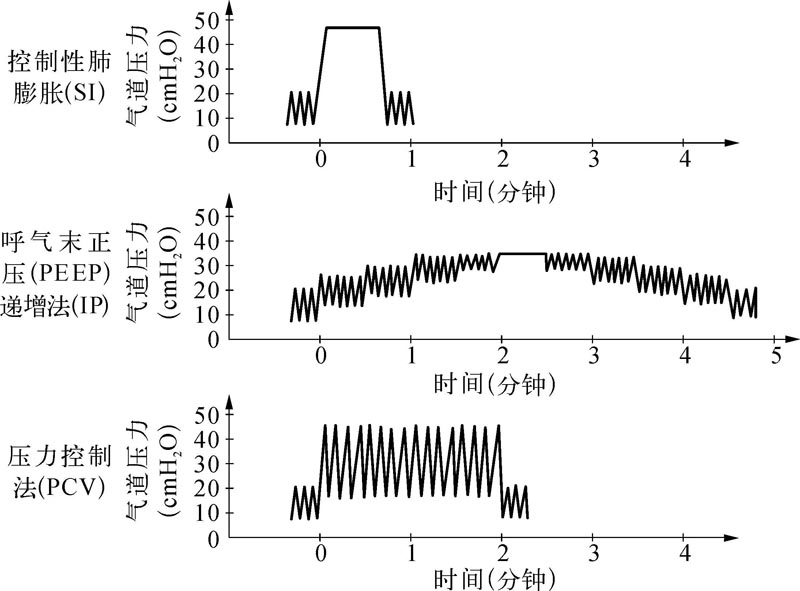
\includegraphics{./images/Image00050.jpg}
 \captionsetup{justification=centering}
 \caption{肺复张手法实施过程压力-时间波形}
 \label{fig5-1}
  \end{figure} 

肺复张手法的效应受多种因素影响。实施肺复张手法的压力和时间设定对肺复张的效应有明显影响,不同肺复张手法效应也不尽相同。另外,ARDS病因不同,对肺复张手法的反应也不同,一般认为,肺外源性的ARDS对肺复张手法的反应优于肺内源性的ARDS;ARDS病程也影响肺复张手法的效应,早期ARDS肺复张效果较好。

\subsubsection{肺复张手法对呼吸和循环系统有何影响?}

在实施肺复张手法的过程中,由于采用了较高复张压力,胸腔内压也随之增加,在短时间内可能产生以下病理生理学影响:①部分肺泡过度膨胀导致局部肺血管阻力增加,产生死腔样通气,同时血液流入充气不良或塌陷的肺泡区域,又导致肺内分流增加;②胸腔内压增加压迫心脏,导致右心房压升高,回心血量减少,心输出量随之下降;③膈肌下移,腹内压增加,阻碍肝脏血流回心。虽然肺复张手法在实施过程中可能产生一些不利的病理生理学改变,但由于肺复张手法实施时间较短,实施肺复张手法后上述病理生理学变化很快消失,所以往往并不产生不良临床后果。

临床上,实施肺复张手法须注意的并发症主要有血流动力学波动及气压伤等。实验及临床研究均显示,肺复张手法实施过程中可导致短时间的血流动力学波动。Lim等的实验研究显示,3种肺复张手法实施过程中均可导致心输出量和平均动脉压的明显下降,但在5~15分钟内可恢复到基础水平
\protect\hyperlink{text00011.htmlux5cux23ch6-10}{\textsuperscript{{[}6{]}}}
。因此,对于基础血流动力学不稳定的患者实施肺复张手法时应格外慎重,必须首先保证充足容量状态。此外,对于肺部感染导致的急性呼吸窘迫综合征,控制性肺膨胀(SI)对心输出量的影响明显高于压力控制通气法,提示对于此类ARDS患者应尽量避免使用控制性肺膨胀方法进行肺复张
\protect\hyperlink{text00011.htmlux5cux23ch6-10}{\textsuperscript{{[}6{]}}}
。复张压力过高可能会导致气压伤,临床上应注意避免复张压力过高,但由肺复张导致的气压伤并不常见。临床上,实施肺复张手法的过程中,如动脉收缩压降低到90mmHg或比复张前下降30mmHg,心率增加到140次/分钟,或比复张前增加20次/分,经皮动脉血氧饱和度降低到90%或比复张前降低5%以上,以及出现新发生心律失常时,应及时终止肺复张。

\subsubsection{急性呼吸窘迫综合征患者机械通气时如何选择适当的呼气末正压?}

肺复张后肺开放效应持续时间主要取决于肺复张后的呼气末正压(PEEP)水平。充分肺复张后,最佳呼气末正压的选择一直是学术界争论的焦点。急性呼吸窘迫综合征(ARDS)广泛肺泡塌陷不但可导致顽固的低氧血症,而且部分可复张的肺泡周期性塌陷开放而产生剪切力,会导致或加重呼吸机相关肺损伤。充分复张塌陷肺泡后应用适当水平呼气末正压可防止呼气末肺泡塌陷,改善低氧血症,并避免剪切力,减轻呼吸机相关肺损伤。因此,ARDS患者机械通气时,应采用能防止肺泡塌陷的最低呼气末正压。

ARDS最佳呼气末正压的选择目前仍存在争议。荟萃分析比较了不同呼气末正压对ARDS患者生存率的影响,结果表明,ARDS早期采用呼气末正压>12cm
H\textsubscript{2} O、尤其是>16cm H\textsubscript{2}
O时明显改善生存率。提示对于ARDS早期患者应采用较高水平的呼气末正压。有学者建议可参照肺静态压力-容积曲线低位转折点压力来选择呼气末正压。Amato及Villar的研究显示,在小潮气量通气的同时,以静态压力-容积曲线低位转折点压力+2cm
H\textsubscript{2}
O作为呼气末正压,结果与常规通气相比ARDS患者的病死率明显降低。因此,若有条件,可根据静态压力-容积曲线低位转折点压力+2cm
H\textsubscript{2}
O来确定呼气末正压。除此之外,还有多种呼气末正压选择方法,如氧合法、最大顺应性法、肺牵张指数法、氧输送法、CT法、依据静态压力-容积曲线吸气支低位拐点或呼气支拐点选择呼气末正压以及根据跨肺压选择呼气末正压等方法。目前,尚无足够的证据支持应采用何种方法选择肺复张后的最佳呼气末正压更为合适,呼气末正压的选择在很大程度上还依赖于临床医师的经验。

\subsubsection{如何描绘肺静态压力-容积曲线?}

常用的肺静态/准静态压力-容积曲线的描绘方法主要分为采点法和连续法。采点法又包括大注射器法和阻塞法等,连续法主要包括体积描记仪法和目前广泛应用的低流速法等。低流速法测定准静态压力-容积曲线是采用非常缓慢的流速描记连续的压力容积曲线,具有简便省时,不需要断开呼吸机等优点。有研究证实,低流速法与经典的大注射器法测定压力-容积曲线一致性良好
\protect\hyperlink{text00011.htmlux5cux23ch17-10}{\textsuperscript{{[}17{]}}}
。低流速法测定压力-容积曲线时,首先应将患者充分镇静和肌松以消除自主呼吸的影响。充分供氧后,将呼吸机调整为容量控制模式,采用高潮气量(如15ml/kg)、低流速(如5~10L/分钟)、低呼吸频率(5次/分钟左右)通气一次或数次,用呼吸机或呼吸功能监护仪描记压力-容积曲线,即为准静态压力-容积曲线。

\subsubsection{如何测定肺静态压力-容积曲线的低位转折点?有何临床意义?}

急性呼吸窘迫综合征(ARDS)患者的肺静态压力-容积曲线吸气支通常为“S”形,低位转折点(lower
inflection
point,LIP)是压力-容积曲线吸气支的低肺容积处出现的一个转折点(图\ref{fig5-2})。传统认为低位转折点表示大部分肺泡开放时对应的压力和容积,现在认为低位转折点可能反映呼气末塌陷的肺泡自此压力开始复张。一些学者主张可用低位转折点对应的压力+2cm
H\textsubscript{2}
O,作为ARDS患者肺复张后的最佳呼气末正压(PEEP)。Amato及Villar的研究显示,在小潮气量通气的同时,以静态压力-容积曲线低位转折点压力+2cm
H\textsubscript{2} O作为PEEP,结果与常规通气相比ARDS患者的病死率明显降低
\protect\hyperlink{text00011.htmlux5cux23ch18-10}{\textsuperscript{{[}18{]}}}
。可见,以低位转折点+2cm H\textsubscript{2}
O确定呼气末正压水平,是ARDS患者肺复张后最佳呼气末正压选择的一种良好方法。

\begin{figure}[!htbp]
 \centering
 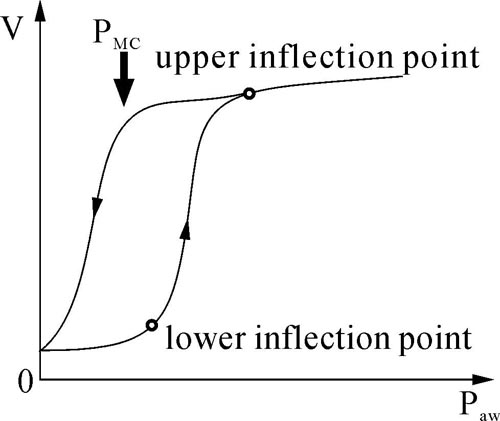
\includegraphics{./images/Image00051.jpg}
 \captionsetup{justification=centering}
 \caption{ARDS患者P-V曲线上低、高拐点及第三拐点}
 \label{fig5-2}
  \end{figure} 

低位转折点的测定包括目测法、顺应性法和双向回归法。目测法最简单但误差较大。顺应性法是将描记压力容积曲线吸气支,依次计算肺顺应性,当顺应性增加了20%提示出现低位转折点。双向回归法是利用计算机软件,用压力-容积曲线上的每一组数据向前和向后做双向直线回归求出相应的回归系数乘积(Ra×Rb),再求出Ra×Rb最大的那一组数据,就是转折点相应的原始数据,然后由这一点分别向前和向后做直线回归,求出它们的斜率(Sa、Sb),再计算出Sb/Sa。下一步求出直线a和直线b的截距,然后计算出各自交点的X和Y值即转折点对应的压力和容积。双向回归法测定低位转折点虽然比较准确,但需要呼吸功能监护仪及特定软件,临床实施有一定难度。

\subsubsection{如何应用氧合法选择最佳呼气末正压?}

氧合法选择最佳呼气末正压(PEEP)是以保持最佳氧合为导向的PEEP选择方法,反映了急性呼吸窘迫综合征(ARDS)机械通气治疗最根本的要求,有学者主张将其作为肺复张后呼气末正压选择的金标准。选择呼气末正压前,应首先进行充分的肺复张,肺复张充分的标准是实施肺复张手法后氧合指数>400mmHg,或两次肺复张后氧合指数的变化<5%。肺复张后直接将呼气末正压设置到较高的水平(如20cm
H\textsubscript{2} O),然后每隔一段时间将呼气末正压降低2cm
H\textsubscript{2}
O,直至氧合指数的降低>5%(提示肺泡重新塌陷),然后重新肺复张后将呼气末正压水平调至氧合指数降低>5%时的呼气末正压+2cm
H\textsubscript{2} O,即为最佳呼气末正压
\protect\hyperlink{text00011.htmlux5cux23ch1-10}{\textsuperscript{{[}1{]}}}
。氧合法选择最佳呼气末正压原理比较简单,但在临床操作上需要反复进行血气分析,在没有持续动脉血氧分压监测的情况下,可行性可能会受到一定限制。

\subsubsection{如何应用最大顺应性法选择最佳呼气末正压?}

最近Henzler等通过CT观察肺复张的效果发现,肺顺应性的变化比动脉氧合和肺内分流能更好地反映复张后肺通气区域与非通气区域的变化。因此,提出以保持最佳肺顺应性为导向的呼气末正压选择方法
\protect\hyperlink{text00011.htmlux5cux23ch19-10}{\textsuperscript{{[}19{]}}}
。具体方法也是在充分肺复张的基础上,首先设定较高的呼气末正压水平(如20cm
H\textsubscript{2}
O),然后逐步缓慢降低呼气末正压水平,同时观察每次呼气末正压调整后的肺动态顺应性变化,直到肺动态顺应性突然下降,然后重新肺复张后将呼气末正压水平调至肺动态顺应性突然下降前的水平。最大顺应性法的实施要求呼吸机具有监测肺动态顺应性的功能,最好能监测每次呼吸肺动态顺应性的变化曲线。

\subsubsection{什么是跨肺压,如何应用跨肺压滴定呼气末正压?}

跨肺压是呼吸运动过程中,扩张肺组织的真正力量。Mead将其定义为在静态条件下作用于胸膜腔表面的对抗肺组织回缩的力量,数值上等于肺组织的弹性回缩力,即肺泡内压与胸膜腔内压的差值。目前临床上多是通过测定食管内压来计算跨肺压。由于静态条件下,气道压等同于肺泡内压,因而,跨肺压的准确测定依赖于胸膜腔内压的测量。胸膜腔内压的测定可以通过将压力传感器放置于胸腔从而直接测量,但是在临床上更多的是通过测量食管内压来代表胸膜腔内压。食管内压的测定是应用带有10cm长气囊的聚氯乙烯导管。通常,食管气囊导管的位置的确定是通过呼气末屏气时自主吸气努力的方法,以确保气囊位于下1/3食管;气囊的充气量则为0.5~1.0ml。已有研究表明,对于直立位的健康志愿者,食管内压可以准确代表胸膜腔内压,从而可以用来计算跨肺压。

当前跨肺压主要用来指导呼气末正压(PEEP)的滴定。食管置管成功后,通过呼气屏气,计算出总呼气末正压与食管内压的差值即跨肺压。因此,如果前次出现的跨肺压<0,通过增加呼气末正压,可使跨肺压逐渐增高,直到跨肺压达到零或者以上,此时对应的呼气末正压就是根据跨肺压滴定出的结果。Talmor初步研究表明,通过测定食管内压控制呼气末跨肺压>0,可以使氧合改善,死腔样通气降低,呼吸系统顺应性改善,甚至出现降低病死率的趋势
\protect\hyperlink{text00011.htmlux5cux23ch20-10}{\textsuperscript{{[}20{]}}}
。因此,通过监测呼气末跨肺压可能有助于急性呼吸窘迫综合征患者个体化的设置呼气末正压水平。

\subsubsection{何为肺牵张指数?有何临床意义?}

肺牵张指数(stress
index)是近年来提出的一项指标,指取容量控制通气恒流的压力-时间曲线吸气支,用曲线回归法算得方程Y=a×t
\textsuperscript{\emph{b}} +c,此\emph{b}
值即为肺牵张指数。肺牵张指数可以反映随着呼气末正压(PEEP)增加,肺泡是不断复张还是过度膨胀。Ranieri等在动物实验中发现,\emph{b}
<1时反映随着吸气潮气量增加,肺泡不断复张,肺顺应性持续增加;\emph{b}
>1时代表随着吸气潮气量增加肺泡过度膨胀,肺顺应性持续降低;\emph{b}
=1对应的是肺泡一直处于开放状态,没有肺泡的塌陷再复张和过度膨胀,避免了塌陷肺泡和细支气管的周期性开放形成的剪切力损伤和肺泡过度扩张导致的过度牵张。此外,Perrot等对移植肺患者的研究显示,用\emph{b}
=1时的呼气末正压进行机械通气,肺损伤程度和局部炎症反应最轻。因此有学者提出,可通过\emph{b}
=1来确定急性呼吸窘迫综合征(ARDS)的患者的呼气末正压水平。

应用肺牵张指数法选择呼气末正压前仍需充分的肺复张。Grasso等用CT证实了肺牵张指数的大小与肺泡塌陷复张和过度膨胀的程度明显相关,但若不用肺复张手法进行肺开放,直接选择肺牵张指数\emph{b}
=1的呼气末正压进行机械通气,此时的呼气末正压明显低于用肺复张手法进行肺开放后选择肺牵张指数\emph{b}
=1的呼气末正压水平,且CT提示仍有大量塌陷的肺泡没有复张
\protect\hyperlink{text00011.htmlux5cux23ch21-10}{\textsuperscript{{[}21{]}}}
。有学者主张,在给予充分复张后,采用较高水平呼气末正压(如20cm
H\textsubscript{2} O)进行容量控制通气,逐渐降低呼气末正压每次2cm
H\textsubscript{2} O,同时测算\emph{b} ,直至\emph{b}
=1,此时的呼气末正压水平即为ARDS患者的最佳呼气末正压。

精确测算\emph{b}
值需用呼吸功能监护仪记录吸气过程的所有压力及其所对应时间,并应用计算机软件计算出\emph{b}
值,步骤繁琐。临床上也可根据容量控制通气压力-时间曲线吸气支的形状来粗略判断\emph{b}
值。如该曲线为一直线则\emph{b} 约为1;如该曲线微向上突起则\emph{b}
<1,反映随着吸气潮气量增加肺泡不断复张,提示呼气末正压可能不足;若该曲线微向下凹陷,则\emph{b}
>1,代表随着吸气潮气量增加肺泡过度膨胀,提示呼气末正压可能过高(图\ref{fig5-3})。此种方法目测\emph{b}
值虽然不够准确,但可操作性好,利于临床应用。

\begin{figure}[!htbp]
 \centering
 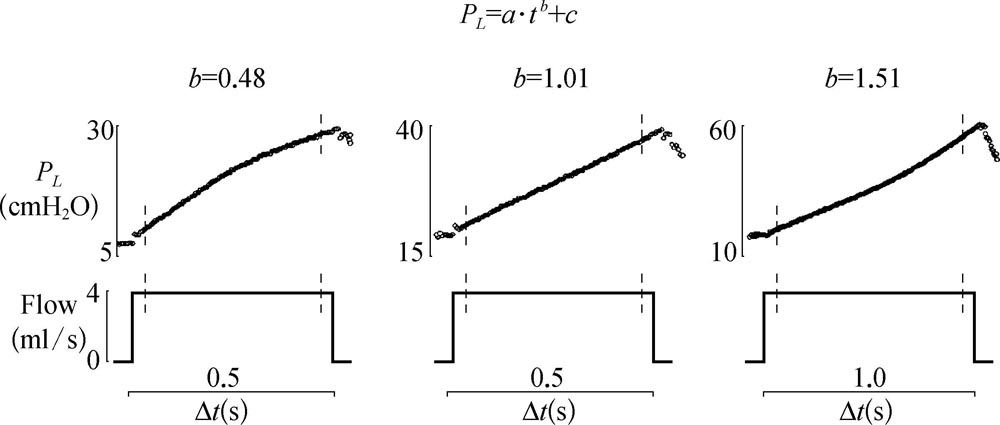
\includegraphics{./images/Image00052.jpg}
 \captionsetup{justification=centering}
 \caption{容量控制通气吸气支形状与肺牵张指数的关系}
 \label{fig5-3}
  \end{figure} 

\subsubsection{什么是肺静态压力-容积曲线第三拐点?意义如何?}

急性呼吸窘迫综合征(ARDS)患者静态压力-容积曲线吸气支通常为“S”形,在低肺容积处和高肺容积处出现的转折分别是低和高拐点,呼气支上出现的转折称为第三拐点(\protect\hyperlink{text00010.htmlux5cux23ck001}{图\ref{fig4-2}}
)。第三拐点测定一般是用大注射器法描记呼气支的曲线,用回归方程计算出第三拐点,而新一代的呼吸机可通过限制呼气流速法描记准静态压力-容积曲线的呼气支,使第三拐点的测定更为简便。目前认为,第三拐点是ARDS呼气时肺泡大量塌陷的开始,反映肺泡的闭合压,而呼气末正压(PEEP)的主要生理学目标是防止ARDS患者呼气末大量的肺泡塌陷,因此,有学者主张应根据第三拐点对应的压力水平设置ARDS患者肺复张后最佳呼气末正压。近期对照实验显示,第三拐点方法选择的呼气末正压水平较氧合法高,平台压有所升高,顺应性有所降低,氧合无明显改变。Takeuchi等研究也提示第三拐点法选择的呼气末正压水平较氧合法高。提示第三拐点方法选择的呼气末正压水平能够维持肺泡持续张开状态,但也可能因气道压过高而导致部分肺泡过度膨胀。目前,第三拐点方法选择最佳呼气末正压受到越来越多学者的关注,但还缺少临床研究证实这种方法的有效性和安全性。

\subsubsection{急性呼吸窘迫综合征患者机械通气时是否需要保留自主呼吸?}

自主呼吸过程中,膈肌主动收缩可增加急性呼吸窘迫综合征(ARDS)患者肺重力依赖区的通气,促进重力依赖区塌陷的肺泡复张,改善通气血流比例失调,进而改善氧合。在患者循环功能稳定,人机协调性较好的情况下,保留自主呼吸的机械通气能更好地改善通气血流比例,从而有可能明显地改善氧合。前瞻对照研究显示,与控制通气相比,保留自主呼吸患者的镇静剂使用量、机械通气时间和住重症医学科时间均明显减少。同时,保留自主呼吸也有利于延缓呼吸机相关的膈肌功能不全的发生。需要注意的是,如果重症ARDS患者自主呼吸很强,吸气时由此产生的胸膜腔内负压增加可能导致跨肺压明显升高,并加重肺损伤。近期研究表明,重症ARDS患者早期(48小时内)在充分镇静剂基础上应用肌松剂可降低患者90天病死率,推测其机制可能与肌松剂减少了人机不同步导致的肺损伤有关
\protect\hyperlink{text00011.htmlux5cux23ch22-10}{\textsuperscript{{[}22{]}}}
。因此,临床上需根据ARDS患者具体情况决定是否应该保留自主呼吸。

\subsubsection{哪些急性呼吸窘迫综合征患者适合应用俯卧位通气?}

俯卧位通气能明显改善急性呼吸窘迫综合征(ARDS)患者的氧合,其机制包括降低胸腔内压力梯度、促进分泌物引流和促进肺内液体移动等。一项随机研究采用每天7小时俯卧位通气,连续7天,结果表明俯卧位通气明显改善大部分ARDS患者氧合,但俯卧位通气对患者病死率无明显影响。然而若依据氧合指数对患者进行分层分析结果显示,氧合指数<88mmHg的患者俯卧位通气后病死率明显降低。此外,依据简化急性生理评分Ⅱ进行分层分析显示,简化的急性生理评分Ⅱ高于49分的患者采用俯卧位通气后病死率显著降低。最近,另外一项每天20小时俯卧位通气的随机对照研究显示,俯卧位通气有降低严重低氧血症患者病死率的趋势。虽然俯卧位通气尚未作为ARDS常规的治疗手段,但对于采用小潮气量通气后气道平台压仍>30cm
H\textsubscript{2}
O的患者应考虑采用俯卧位通气。ARDS患者采用俯卧位通气是比较安全的。在俯卧位前,应考虑患者有否严重的低血压、室性心律失常、颜面部创伤及未处理的不稳定性骨折等俯卧位通气的相对禁忌证。研究报道,体位改变过程中可能发生如气管插管及中心静脉导管意外脱落等并发症,需要予以预防,但严重并发症并不常见。

\subsubsection{半卧位对机械通气急性呼吸窘迫综合征患者有何益处?}

急性呼吸窘迫综合征(ARDS)患者如合并呼吸机相关性肺炎,往往使肺损伤进一步恶化,预防呼吸机相关性肺炎具有重要的临床意义。由于气管插管或气管切开导致声门的关闭功能丧失,平卧位时,机械通气患者胃肠内容物更易反流误吸进入下呼吸道,而导致呼吸机相关性肺炎。研究表明,低于30°角的平卧位是院内获得性肺炎的独立危险因素。前瞻性随机对照研究显示,机械通气患者平卧位和半卧位(头部抬高45°以上)呼吸机相关性肺炎的患病率分别为34%和8%(\emph{P}
=0.003),经微生物培养确诊的呼吸机相关性肺炎患病率分别为23%和5%(\emph{P}
=0.018)。可见,半卧位可显著降低机械通气患者呼吸机相关性肺炎的发生。因此,除非有脊髓损伤等体位改变的禁忌证,机械通气患者均应保持30°~45°的半卧位,以预防呼吸机相关性肺炎的发生
\protect\hyperlink{text00011.htmlux5cux23ch23-10}{\textsuperscript{{[}23{]}}}
。

\subsubsection{气道压力释放通气对急性呼吸窘迫综合征治疗有何价值?}

气道压力释放通气是通过周期性地释放压力以减少肺容量而排出二氧化碳,当释放活瓣重新关闭后,呼吸机迅速充气恢复至预置的高气道压水平,此时患者在较高水平的功能残气量位自主呼吸。气道压力释放通气的通气目标是限制气道峰压,减少气压伤和心血管受损,改善氧合和通气/血流比例。急性呼吸窘迫综合征(ARDS)患者实施气道压力释放通气过程中,由于气道压力释放的时间较短,避免了肺泡塌陷,可能有助于改善氧合和通气/血流比例,进而改善ARDS患者的氧合。研究证实,与压力控制通气相比,气道压力释放通气可明显改善ARDS患者的氧合。因此,对常规肺保护性通气仍不能维持氧合的ARDS患者,可考虑应用气道压力释放通气。

\subsubsection{高频振荡通气在急性呼吸窘迫综合征治疗中有何优势?}

高频振荡通气通过往复运动的活塞泵、扬声器隔膜或旋转球的方式产生正弦波,使气管内气体产生高频往返运动,将气体主动送入和吸出气道。急性呼吸窘迫综合征(ARDS)患者实施高频振荡通气过程中,应用一定水平的驱动压(即气道平均压),可保持肺泡持续处于膨胀状态,避免了常规通气模式呼气时的肺泡塌陷,避免了肺泡反复塌陷复张导致的肺损伤,同时也避免了由于部分肺泡塌陷所致的肺内分流,有助于改善ARDS患者氧合。动物实验显示,在气道平均压相同的情况下,与传统通气模式相比,高频振荡通气时,气道抽吸物中炎症介质水平明显降低。非随机临床研究显示,常规通气无效的严重ARDS患者改用高频振荡通气后,氧合明显改善,心输出量和氧输送无明显改善,提示对于严重ARDS患者,高频振荡通气是一种有效且安全的通气模式。2002年一项多中心随机对照研究显示,与常规通气相比,高频振荡通气的ARDS患者的氧合改善更早(机械通气16小时以内),但在24小时时两种通气模式的氧合无显著差异,高频振荡通气组30天病死率有下降趋势(37%对比52%,\emph{P}
=0.102)。

高频振荡通气是重症ARDS肺保护性通气方式的选择之一,有利于采用更小的潮气量,控制平台压力,改善严重低氧血症患者的氧合,但对重症ARDS患者病死率的影响仍需大规模的临床研究。高频振荡通气尚不能作为ARDS的常规通气模式,对于积极的肺复张实施后仍难以改善其低氧血症,且采用小潮气量通气后气道平台压仍>30cm
H\textsubscript{2} O的患者可考虑应用高频振荡通气。

\subsubsection{何为液体通气?对急性呼吸窘迫综合征的治疗效果如何?}

以液体作为携氧介质输入肺内进行机械通气即为液体通气,其研究始于20世纪60年代。1966年Clark等发现强大携氧能力的高氟碳化合物,并将实验动物浸没其中进行气体交换取得成功,从而揭开了液体通气技术研究的新篇章。1996年Hirsch首次将液体通气技术应用于成人的急性呼吸窘迫综合征(ARDS)患者,在使用液体通气技术后生理分流平均值从0.72降至0.46,同时肺顺应性从0.16增至0.27ml/cm
H\textsubscript{2}
O,50%患者存活,开始了部分液体通气在ARDS患者中的治疗研究。

高氟碳化合物的比重较高,达到11.9kg/cm\textsuperscript{3}
,表面张力仅相当于水的1/4,携氧能力强,极少量通过肺泡吸收入血,在体内几乎不被代谢,而通过肺部蒸发为气体呼出,高氟碳化合物对人体没有任何副作用,这些独特的物理性质是发挥它作为呼吸介质的理论基础。

液体通气治疗ARDS的主要原理为------①改善气体交换:高氟碳化合物具有较高的携氧和二氧化碳的能力,可起到“液态(PEEP)”效应,使萎陷的肺泡得以重新开放,降低肺泡表面张力、减少死腔,此外,高氟碳化合物比重较高,在重力作下用,使肺内上下区域的血流得到重新分布,尤其是使肺下垂部位的血流相对减少,改善肺内通气/血流比例,进而改善氧合;②改善肺顺应性:高氟碳化合物能使原来的气液-界面改变成液-液界面,从而降低了表面张力,加上高氟碳化合物本身就具有较低的表面张力,有类似表面活性物质作用可以使肺泡复张并降低肺泡表面张力,改善顺应性;③抗炎作用:高氟碳化合物有直接抗炎作用,研究发现,暴露在高氟碳化合物中的巨噬细胞产生的过氧化氢和氧自由基减少。高氟碳化合物也有间接抗炎作用。高氟碳化合物因其密度高且不与亲水性物质相溶,沉积于肺泡内炎性渗出物与肺泡上皮之间,可形成一层保护屏障,有利于炎性渗出物排出。

部分液体通气是在常规机械通气的基础上经气管插管向肺内注入相当于功能残气量的全氟碳化合物,以降低肺泡表面张力,促进肺重力依赖区塌陷肺泡复张。研究显示,部分液体通气72小时后,ARDS患者肺顺应性可以得到改善,并且改善气体交换,对循环无明显影响,但患者预后均无明显改善,病死率仍高达50%左右。近期对90例ARDS患者的随机对照研究显示,与常规机械通气相比,部分液体通气既不缩短机械通气时间,也不降低病死率;进一步分析显示,对于年龄<55岁的患者,部分液体通气有缩短机械通气时间的趋势。总之,部分液体通气能改善ARDS患者气体交换,增加肺顺应性,可作为严重ARDS患者常规机械通气无效时的一种选择。

\subsubsection{重症ARDS危及生命低氧血症治疗的策略是什么?}

2010年Janet等在《Critical Care
Medicine》杂志发表继续教育综述,将重症ARDS危及生命低氧血症治疗的策略总结为6个步骤,有学者称之为ARDS治疗六步法(图\ref{fig5-4})
\protect\hyperlink{text00011.htmlux5cux23ch24-10}{\textsuperscript{{[}24{]}}}
。包括如下步骤:

\begin{figure}[!htbp]
 \centering
 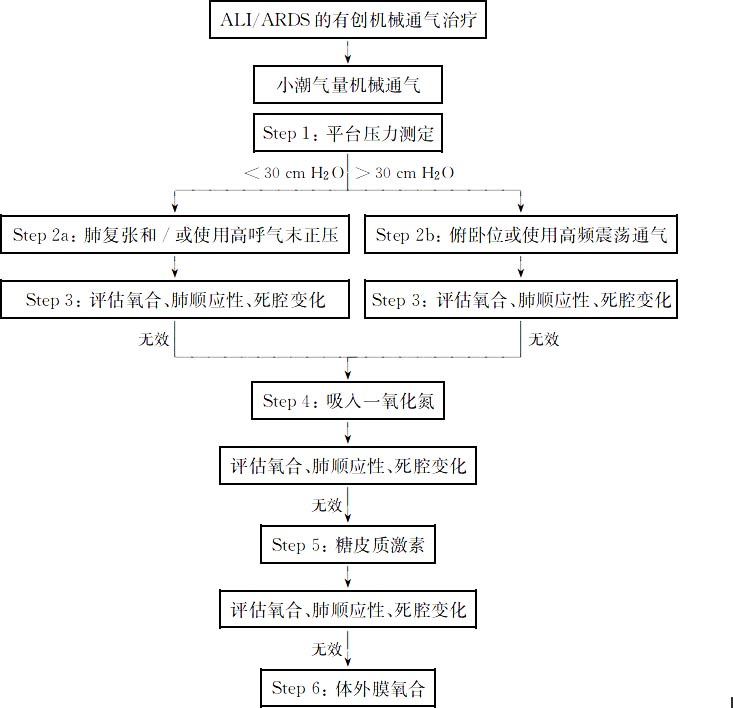
\includegraphics{./images/Image00053.jpg}
 \captionsetup{justification=centering}
 \caption{重症急性呼吸窘迫综合征治疗六步法}
 \label{fig5-4}
  \end{figure} 

步骤1.测量气道平台压力,如果<30cm H\textsubscript{2}
O,进入步骤2a。如果>30cm H\textsubscript{2} O,进入步骤2b。

步骤2a.实施肺复张和(或)使用高呼气末正压。

步骤2b.实施俯卧位通气或高频振荡通气。

步骤3.评价氧合改善效果、静态顺应性和死腔通气,如果改善明显则继续治疗;如果改善不明显,则进入下一步。

步骤4.给予吸入一氧化氮治疗,如果几小时内没有反应,则进入下一步。

步骤5.给予糖皮质激素治疗,个体化评价患者的风险与收益。

步骤6.考虑实施体外生命支持,入选者高压通气时间须短于7天。

每一步骤实施后,都应仔细评价氧合改善效果、静态顺应性和死腔通气。如果改善明显则继续治疗。如果改善不明显,则进入下一步。

\subsection{急性呼吸窘迫综合征的药物治疗}

\subsubsection{哪些急性呼吸窘迫综合征患者适于应用糖皮质激素治疗?}

全身和局部的炎症反应是急性呼吸窘迫综合征(ARDS)发生和发展的重要机制,研究显示,血浆和肺泡灌洗液中的炎症因子浓度升高与ARDS病死率呈正相关。长期以来,大量的研究试图应用糖皮质激素控制炎症反应,预防和治疗ARDS。早期的3项多中心随机对照研究观察了大剂量糖皮质激素对ARDS的预防和早期治疗作用,结果糖皮质激素既不能预防ARDS的发生,对早期ARDS也没有治疗作用。ARDS患者是否常规应用应激剂量的糖皮质激素仍有争议,但对于过敏原因导致的ARDS患者,早期应用糖皮质激素经验性治疗可能有效。此外,感染性休克并发ARDS的患者,或合并有肾上腺皮质功能不全,也可考虑应用替代剂量的糖皮质激素。对于H1N1流感病毒感染导致的ARDS,激素治疗可能并无益处。

持续的过度炎症反应和肺纤维化是导致ARDS晚期病情恶化和治疗困难的重要原因。糖皮质激素能抑制ARDS晚期持续存在的炎症反应,并能防止过度的胶原沉积,从而有可能对晚期ARDS有保护作用。小样本随机对照试验显示,对于治疗1周后未好转的ARDS患者,糖皮质激素治疗组的病死率明显低于对照组,感染发生率与对照组无差异,高血糖发生率低于对照组。然而,最近ARDSnet的研究观察了糖皮质激素对晚期ARDS(患病7~24天)的治疗效应
\protect\hyperlink{text00011.htmlux5cux23ch25-10}{\textsuperscript{{[}25{]}}}
,结果显示,糖皮质激素治疗(甲基泼尼松龙每天2mg/kg,分4次静脉点滴,14天后减量)并不降低60天病死率,但可明显改善低氧血症和肺顺应性,缩短患者的休克持续时间和机械通气时间。进一步亚组分析显示,ARDS发病>14天应用糖皮质激素会明显增加病死率。可见,对于晚期ARDS患者不宜常规应用糖皮质激素治疗。

\subsubsection{急性呼吸窘迫综合征患者为何要实施限制性液体管理的策略?}

高通透性肺水肿是急性呼吸窘迫综合征(ARDS)的病理生理特征,肺水肿的程度与ARDS的预后呈正相关,因此,通过积极的液体管理,改善ARDS患者的肺水肿具有重要的临床意义。

研究显示液体负平衡与感染性休克患者病死率的降低显著相关,且对于创伤导致的ARDS患者,液体正平衡使患者病死率明显增加。应用利尿剂减轻肺水肿可能改善肺部病理情况,缩短机械通气时间,进而减少呼吸机相关性肺炎等并发症的发生。但是利尿减轻肺水肿的过程可能会导致心输出量下降,器官灌注不足。因此,ARDS患者的液体管理必需考虑到二者的平衡,必须在保证脏器灌注的前提下进行。

最近,ARDSnet完成的不同ARDS液体管理策略的研究显示
\protect\hyperlink{text00011.htmlux5cux23ch21-10}{\textsuperscript{{[}21{]}}}
,尽管限制性液体管理与非限制性液体管理组病死率无明显差异,但与非限制性液体管理相比,限制性液体管理(利尿和限制补液)组患者第1周的液体平衡为负平衡(-136ml对比+6992ml),氧合指数明显改善,肺损伤评分明显降低,而且重症医学科住院时间明显缩短。特别值得注意的是,限制性液体管理组的休克和低血压的发生率并无增加。可见,在维持循环稳定、保证器官灌注的前提下,限制性的液体管理策略对ARDS患者是有利的。

\subsubsection{急性呼吸窘迫综合征患者应采用晶体液还是胶体液进行复苏?}

急性呼吸窘迫综合征(ARDS)患者采用晶体液还是胶体液进行液体复苏一直存在争论。ARDS的基本病理生理改变是高通透性肺水肿,有学者认为,用胶体液进行复苏可提高血浆胶体渗透压,缓解肺血管渗漏和肺水肿,可能对ARDS患者有益。但最近的大规模随机对照研究显示,应用白蛋白进行液体复苏,在改善生存率、脏器功能保护、机械通气时间及重症医学科住院时间等方面与生理盐水无明显差异。因此,目前尚无证据支持在ARDS患者液体复苏时采用胶体液优于晶体液。

值得注意的是,胶体渗透压是决定毛细血管渗出和肺水肿严重程度的重要因素。研究证实,低蛋白血症是严重感染患者发生ARDS的独立危险因素,而且低蛋白血症可导致ARDS病情进一步恶化,并延长机械通气时间,病死率也明显增加。因此,对低蛋白血症的ARDS患者,有必要输入白蛋白或人工胶体,提高胶体渗透压。最近两个多中心随机对照研究显示,对于存在低蛋白血症(血浆总蛋白<50~60g/L)的ARDS患者,与单纯应用呋塞米(速尿)相比,尽管白蛋白联合速尿治疗未能明显降低病死率,但可明显改善氧合、增加液体负平衡,并缩短休克时间。因此,对于存在低蛋白血症的ARDS患者,在补充白蛋白等胶体溶液的同时联合应用呋塞米,有助于实现液体负平衡,并改善氧合。人工胶体对ARDS是否也有类似的治疗效应,需进一步研究证实。

\subsubsection{吸入一氧化氮纠正急性呼吸窘迫综合征低氧血症的机制是什么?}

一氧化氮吸入可选择性扩张肺血管,而且吸入一氧化氮分布于肺内通气良好的区域,可扩张该区域的肺血管,显著降低肺动脉压,减少肺内分流,改善通气/血流比例失调,并且可减少肺水肿形成,已成为急性呼吸窘迫综合征(ARDS)重要的呼吸支持治疗措施之一。一氧化氮改善低氧血症的主要机制包括:①ARDS导致的低氧血症可引起肺毛细血管痉挛,一氧化氮吸入治疗时,通气正常或接近正常的肺泡中一氧化氮浓度较高,使其周围痉挛的毛细血管扩张,灌注改善,通气不佳区域的血流向该区域转移,结果是通气好的区域通气/血流比例改善,通气不良区域肺内分流减少,进而改善氧合;②通气不良的肺泡中一氧化氮浓度较低,一氧化氮对肺毛细血管的影响较小,不会引起肺内分流增加;③一氧化氮可部分改善小气道痉挛,改善肺泡通气,进一步减少肺内分流。

临床上一氧化氮吸入可使约60%的ARDS患者氧合改善,同时肺动脉压、肺内分流明显下降,但对平均动脉压和心输出量无明显影响。氧合改善效果一般仅限于开始一氧化氮吸入治疗的24~48小时内。两个随机对照研究证实一氧化氮吸入并不能改善ARDS的病死率。目前,吸入一氧化氮并不是ARDS的常规治疗手段,鉴于吸入一氧化氮能改善顽固性低氧血症,降低呼吸机条件和吸入氧浓度,在一般治疗无效的严重低氧血症时可应用,可能减少医源性肺损伤,并为治疗赢得宝贵的时间。

\subsubsection{如何评价肺泡表面活性物质对急性呼吸窘迫综合征的治疗价值?}

急性呼吸窘迫综合征(ARDS)患者存在肺泡表面活性物质减少或功能丧失,故而易引起肺泡塌陷。肺泡表面活性物质能降低肺泡表面张力,减轻肺炎症反应,阻止氧自由基对细胞膜的氧化损伤。因此,补充肺泡表面活性物质可能成为ARDS的治疗手段。但是,早期的随机对照研究显示,应用肺泡表面活性物质后,ARDS患者的血流动力学指标、动脉氧合、机械通气时间、重症医学科住院时间和30天生存率并无明显改善。有学者认为阴性结果可能与表面活性物质剂量不足有关。随后的小样本剂量对照研究显示,与安慰剂组及肺泡表面活性物质50mg/kg应用4次组比较,100mg/kg应用4次和8次,有降低ARDS28天病死率的趋势(43.8%、50%对比18.8%、16.6%,\emph{P}
=0.075)。2004年有两个中心参加的随机对照研究显示,补充肺泡表面活性物质能够短期内(24小时)改善ARDS患者的氧合,但并不影响机械通气时间和病死率。最近一项针对心脏手术后发生ARDS补充肺泡表面活性物质的临床研究显示,与既往病例比较,治疗组氧合明显改善,而且病死率下降。目前肺泡表面活性物质的应用仍存在许多尚未解决的问题,如最佳用药剂量、具体给药时间、给药间隔和药物来源等。因此,尽管早期补充肺表面活性物质有助于改善氧合,但目前还不能将其作为ARDS的常规治疗手段。如今进一步研究肺泡表面活性物质的用法,并明确其对ARDS预后的影响显得非常必要。

\subsubsection{β2 受体激动剂治疗急性呼吸窘迫综合征患者有效吗?}

β\textsubscript{2}
受体激动剂治疗急性呼吸窘迫综合征(ARDS)患者的理论依据包括:①减少中性粒细胞的激活和聚集,并且减少炎症因子的产生;②通过激活Ⅰ型和Ⅱ型肺泡上皮细胞β\textsubscript{2}
受体,增加细胞内环磷腺苷(cAMP),促进细胞内外钠离子的转移,从而达到清除肺水的目的。

2007年美国ARDSnet进行的前瞻性、随机、双盲对照研究(ALTA研究)采用吸入β\textsubscript{2}
受体激动剂治疗ARDS,在2009年因无效被数据监测委员会终止。而在英国进行的另一项多中心、双盲、随机平行对照研究(BALTI-2研究),观察静脉注射沙丁胺醇是否能降低ARDS患者28天病死率,发现虽然治疗组无机械通气时间和无器官功能衰竭时间明显减少,但沙丁胺醇引起的重症医学科住院患者病死率增加8.4%(95%CI-1.7-18.3),住院病死率也增加6%(95%CI-4.4-16.2)
\protect\hyperlink{text00011.htmlux5cux23ch26-10}{\textsuperscript{{[}26{]}}}
。目前研究显示雾化吸入或静脉使用沙丁胺醇并不能使早期ARDS患者受益,反而可能会增加病死率,所以对于机械通气的ARDS患者不推荐常规使用β\textsubscript{2}
受体激动剂治疗。

\subsubsection{重症急性呼吸窘迫综合征患者如何应用神经肌肉阻滞剂?}

神经肌肉阻滞药(neuromuscular blocking
agents,NMBAs)亦称骨骼肌松弛药(muscular
relaxants),简称肌松药。近期20个研究中心通过前瞻性随机双盲对照试验证实,与安慰剂组比较,重症急性呼吸窘迫综合征(ARDS)患者早期(48小时内)在充分镇静剂基础上应用顺式阿库溴铵治疗可降低90天病死率,缩短机械通气时间,减缓器官功能衰竭的发生,缩短90天内重症医学科住院日并降低气胸发生率。肌松剂改善重症ARDS患者预后可能的机制包括:促进人机协调;改善氧合;拮抗肺部和全身炎症反应;降低氧消耗;预防或减轻呼吸机诱导性肺损伤。应用肌松药的主要安全担忧是导致获得性肌病。但上述研究结果显示
\protect\hyperlink{text00011.htmlux5cux23ch22-10}{\textsuperscript{{[}22{]}}}
,肌松药与安慰剂组间的重症医学科获得性肌无力发生率无显著差别。对于重症ARDS患者的早期阶段,可考虑短期应用神经肌肉阻滞剂以利于肺保护性通气策略的实施。

\subsection{急性呼吸窘迫综合征的预防}

\subsubsection{术中限制性液体管理可预防急性呼吸窘迫综合征的发生吗?}

感染、手术、创伤等激活炎症反应,导致高通透性肺水肿,是急性呼吸窘迫综合征(ARDS)发生发展的重要病理生理机制。通过合理的液体管理预防高危患者发生急性肺损伤逐步受到关注。

限制性液体管理有助于预防ARDS的发生。近期Christopher
G等发表回顾性队列研究,旨在探讨术中液体管理与ARDS发生间的关系。研究纳入术后一周内发生急性呼吸衰竭需要机械通气的患者89例,25例发展为ARDS。结果显示术中液体的输注量与ARDS的发生显著相关。与输液量每小时10mL/kg的患者相比,术中接受每小时10~20mL/kg输液量患者的ARDS发生风险增加2.4倍(\emph{P}
<0.14),而>每小时20mL/kg输液量则使ARDS发生风险进一步增加,达3.8倍(\emph{P}
<0.04)
\protect\hyperlink{text00011.htmlux5cux23ch27-10}{\textsuperscript{{[}27{]}}}
。提示临床治疗中需关注液体复苏量对高危患者发生ARDS的影响。在维持循环稳定、保证器官灌注的前提下,限制性的液体管理策略有利于预防高危患者ARDS的发生和发展。

\subsubsection{抗血小板聚集可预防急性呼吸窘迫综合征的发生吗?}

免疫细胞的聚集和活化导致肺泡-毛细血管损伤是急性呼吸窘迫综合征(ARDS)发生发展的根本机制。细胞聚集和损伤激活凝血系统进一步促进肺损伤的发生和发展。

抗血小板聚集抑制凝血系统和血栓形成,有利于维持肺泡毛细血管的通畅性,发挥肺保护作用。阿司匹林是冠心病患者抗凝治疗的常用药物,不仅有助于预防心血管事件的发生,可能还有助于预防ARDS。新近发表的队列研究以入住内科重症医学科、存在ARDS高危因素的患者为研究对象,比较是否服用阿司匹林(住院前及住院时)抗凝与ARDS发生的关系。研究纳入患者161例,79例(49%)接受抗凝治疗。发生急性肺损伤/ARDS的患者共33例(21%),进行抗血小板聚集治疗的患者显著低于无抗凝治疗的患者(12.7%对比28.0%,\emph{P}
<0.02)
\protect\hyperlink{text00011.htmlux5cux23ch28-10}{\textsuperscript{{[}28{]}}}
。提示抗血小板聚集治疗有助于预防ARDS的发生。

\subsubsection{他汀类药物对急性呼吸窘迫综合征有何影响?}

他汀类药物是临床常规使用的降脂药物。近些年来,他汀类药物降脂以外的作用越来越受到重视,尤其值得关注的是其对炎症反应的调控作用、对血管内皮的保护作用和抑制血栓形成的作用。失控的炎症反应和血管内皮损伤是急性呼吸窘迫综合征(ARDS)发生和发展的根本机制,他汀类药物对ARDS的预防和治疗作用成为新近研究的重要方向之一。

近年来,动物和临床实验研究显示他汀类药物具有肺保护作用。动物实验表明他汀类药物通过抑制内皮细胞一氧化氮合酶活性、抑制白细胞粘附和自由基生成预防急性肺损伤的发生和发展
\protect\hyperlink{text00011.htmlux5cux23ch29-10}{\textsuperscript{{[}29{]}}}
\textsuperscript{,}
\protect\hyperlink{text00011.htmlux5cux23ch30-10}{\textsuperscript{{[}30{]}}}
。近期的临床研究观察服用他汀类药物和阿司匹林对ARDS的预防作用,研究纳入患者575例,结果显示服用药物组严重的全身性感染、ARDS发生率和病死率均明显降低
\protect\hyperlink{text00011.htmlux5cux23ch31-10}{\textsuperscript{{[}31{]}}}
,显示他汀类药物和阿司匹林具有肺保护作用。

\subsubsection{胺碘酮与急性呼吸窘迫综合征的发生有何关系?}

胺碘酮是经典的Ⅲ类抗心律失常药物,主要用于治疗室上性和室性快速性心律失常。在发挥治疗作用的同时,临床治疗中必须关注其对肺、甲状腺、皮肤、肝脏等的副作用。

胺碘酮可导致包括急性呼吸窘迫综合征(ARDS)在内的多种肺部并发症。最早认识的胺碘酮肺部并发症是肺纤维化。上世纪90年代,有观察和研究显示合并高浓度氧疗的心胸外科术后患者,应用胺碘酮治疗后ARDS的发生率明显增高。胺碘酮的急性肺损伤/ARDS并发症开始受到关注。随后的研究报道胺碘酮并发ARDS的发生率达9%~50%。

多种高危因素影响胺碘酮肺部ARDS并发症的发生和发展。年龄是发生胺碘酮肺部并发症的独立危险因素。与60岁以下的患者相比,>60岁的患者,年龄每增长10岁,胺碘酮肺部并发症的发生增加3倍。另一影响因素是胺碘酮的使用时间、使用剂量和累积剂量。近年研究表明,胺碘酮持续应用6~12个月、维持剂量200mg/天以上、累积剂量达到10~15g患者随时有出现肺部并发症的风险。维持剂量500mg/天肺部并发症的风险明显高于300mg/天;连续应用1、3、5年,随着累积剂量的增加,肺部并发症的发生率从4.2%、7.8%到10.6%逐步增加。大多研究显示,已存在肺部疾病的患者易出现胺碘酮的肺部并发症,但对患者的病死率没有明显影响
\protect\hyperlink{text00011.htmlux5cux23ch32-10}{\textsuperscript{{[}32{]}}}
。

因此,对于采用胺碘酮抗心律失常治疗的高危患者,须关注药物使用时间、使用剂量和累积剂量对肺损伤的影响,尤其对于存在基础肺疾病的患者,须控制胺碘酮的使用时间、使用剂量和累积剂量,以预防ARDS的发生和发展。

\subsubsection{潮气量设置对急性呼吸窘迫综合征的发生有何影响?}

机械通气是呼吸支持或呼吸治疗的重要手段,但应用不当,尤其是潮气量设置不当,可产生呼吸机相关肺损伤,其本质即为急性呼吸窘迫综合征(ARDS)。防止潮气量损伤成为预防ARDS发生的一个重要环节。

非ARDS机械通气患者的潮气量设置,近年来不断受到关注。荟萃分析表明,围手术期的机械通气患者采用较小潮气量通气,ARDS的发生率显著降低。除此之外,机械通气的呼吸频率影响肺损伤的产生。以Ⅰ型肺泡上皮细胞为研究对象,观察不同牵张幅度和牵张频率的影响,结果显示牵张幅度过高,增加牵张频率加重机械通气所致肺损伤;而牵张幅度较小,即使增加牵张频率也不产生机械通气损伤
\protect\hyperlink{text00011.htmlux5cux23ch33-10}{\textsuperscript{{[}33{]}}}
。新近的RCT研究进一步比较了10ml/kg和6ml/kg理想体重的潮气量对非急性肺损伤(ALI)患者炎症反应和急性肺损伤发生的影响。共纳入患者150例,10ml/kg潮气量组全身和肺部炎症反应明显增加,研究由于该组ARDS的发生率显著升高而被迫提前终止。多元回归分析显示潮气量和呼气末正压的设置是发生急性肺损伤的独立危险因素
\protect\hyperlink{text00011.htmlux5cux23ch34-10}{\textsuperscript{{[}34{]}}}
。上述研究均显示较小潮气量通气对正常肺组织的肺保护作用。

可见,对于非ARDS患者,即使应用常规潮气量通气也不能防止ARDS的发生。采用低于常规潮气量进行机械通气、并防止通气期间的肺泡塌陷,是预防ARDS的重要环节和手段。

临床治疗中,应关注液体管理、机械通气潮气量、药物治疗等对ARDS发生发展的影响。限制性液体管理、较小潮气量通气、抗血小板聚集和他汀类药物发挥肺保护作用,是预防ARDS的关键因素,应用胺碘酮期间,须监测药物对ARDS的影响。

\begin{center}\rule{0.5\linewidth}{\linethickness}\end{center}

参考文献

\protect\hyperlink{text00011.htmlux5cux23ch1-10-back}{{[}1{]}} .Bernard
GR,Artigas A,Brigham KL,et al.The American-European Consensus
Conference on ARDS,definitions,mechanisms,relevant outcomes,and
clinical trial coordination.Am J Respir Crit Care
Med,1994,149:818-824.

\protect\hyperlink{text00011.htmlux5cux23ch2-10-back}{{[}2{]}}
.Rubenfeld GD,Caldwell E,Peabody E,et al.Incidence and outcomes of
acute lung injury.N Engl J Med,2005,353:1685-1693.

\protect\hyperlink{text00011.htmlux5cux23ch3-10-back}{{[}3{]}}
.Lewandowski K,Lewandowski M.Epidemiology of ARDS.Minerva
Anestesiol,2006,72:473-477.

\protect\hyperlink{text00011.htmlux5cux23ch4-10-back}{{[}4{]}} .Phua
J,Badia JR,Adhikari NKJ,et al.Has Mmortality from acute respiratory
distress syndrome decreased over time?:A systematic
review.Am.J.Respir.Crit.Care Med,2009;179:220-227.

\protect\hyperlink{text00011.htmlux5cux23ch5-10-back}{{[}5{]}} .Lu
Y,Song Z,Zhou X,et al.A 12-month clinical survey of incidence and
outcome of acute respiratory distress syndrome in Shanghai intensive
care units.Intensive Care Med,2004,30:2197-2003.

\protect\hyperlink{text00011.htmlux5cux23ch6-10-back}{{[}6{]}} .Lim
SC,Adama AB,Simonson DA,et al.Intercomparison of recruitment
maneuver efficacy in three models of acute lung injury.Crit Care
Med,2004,32:2371-2377.

\protect\hyperlink{text00011.htmlux5cux23ch7-10-back}{{[}7{]}} .Peek
GJ,Mugford M,Tiruvoipati R,et al.Efficacy and economic assessment of
conventional ventilatory support versus extracorporeal membrane
oxygenation for severe adult respiratory failure(CESAR):a multicentre
randomised controlled trial.Lancet.2009,374:1351-1363.

\protect\hyperlink{text00011.htmlux5cux23ch8-10-back}{{[}8{]}} .Gong
MN,Wei Z,Xu LL,et al.Polymorphism in the surfactant protein-B
gene,gender,and the risk of direct pulmonary injury and
ARDS.Chest,2004,125:203-211.

\protect\hyperlink{text00011.htmlux5cux23ch9-10-back}{{[}9{]}} .Quasney
MW,Waterer GW,Dahmer MK,et al.Association between surfactant protein
B+1580 polymorphism and the risk of respiratory failure in adults with
community acquired pneumonia.Crit Care Med,2004,32:1115-1159.

\protect\hyperlink{text00011.htmlux5cux23ch10-10-back}{{[}10{]}} .Lmai
Y,Kuba K,Rao S,et al.Angiotensin-converting enzyme 2 protects from
sever acute lung failure.Nature,2005,436:112-116.

\protect\hyperlink{text00011.htmlux5cux23ch11-10-back}{{[}11{]}}
.Marshall RP,Webb S,Bellingan GJ,et al.Angiotensin converting
enzyme insertion/deletion polymorphism is associated with susceptibility
and outcome in acute respiratory distress syndrome.Am J Crit Care
Med,2002,166:646-650.

\protect\hyperlink{text00011.htmlux5cux23ch12-10-back}{{[}12{]}} .Mira
JP,Cariou A,Grall F,et al.Association of TNF\textsubscript{2} ,a
TNF-alpha promoter polymorphism with septic shock susceptibility
mortality:A multicenter study.JAMA,1999,282:561-568.

\protect\hyperlink{text00011.htmlux5cux23ch13-10-back}{{[}13{]}}
.Marshall RP,Webb S,Hill MR,et al.Genetic polymorphisms associated
with susceptibility and outcome in ARDS.Chest,2002,121:s68-s69.

\protect\hyperlink{text00011.htmlux5cux23ch14-10-back}{{[}14{]}} .The
ARDS Definition Task Force.Acute respiratory distress syndrome the
Berlin definition.JAMA,2012;307:doi:10.1001/jama.2012.5669

\protect\hyperlink{text00011.htmlux5cux23ch15-10-back}{{[}15{]}} .Zhan
Q,Sun B,Liang L,et al Early use of noninvasive positive pressure
ventilation for acute lung injury:A multicenter randomized controlled
trial.Crit Care Med 2012,40:455-460.

\protect\hyperlink{text00011.htmlux5cux23ch16-10-back}{{[}16{]}}
.郭凤梅,邱海波,谭焰,等.低流速法测定急性呼吸窘迫综合征静态肺压力容积曲线的比较性实验研究.中华结核和呼吸杂志,2001,12:728-731.

\protect\hyperlink{text00011.htmlux5cux23ch17-10-back}{{[}17{]}}
.Villar J,Kacmarek RM,Perez-Mendez L,et al.A high positive
end-expiratory pressure,low tidal volume ventilatory strategy improves
outcome in persistent acute respiratory distress syndrome:a
randomized,controlled trial.Crit Care Med,2006,34:1311-1318.

\protect\hyperlink{text00011.htmlux5cux23ch18-10-back}{{[}18{]}}
.Henzler D,Pelosi P,Dembinski R,et al.Respiratory compliance but
not gas exchange correlates with changes in lung aeration after a
recruitment maneuver:an experimental study in pigs with saline lavage
lung injury.Crit Care,2005,9:R471-482.

\protect\hyperlink{text00011.htmlux5cux23ch19-10-back}{{[}19{]}}
.Grasso S,Terragni P,Mascia L,et al.Airway pressure-time curve
profile(stress index)detects tidal recruitment/hyperinflation in
experimental acute lung injury.Crit Care Med,2004,32:1018-1027.

\protect\hyperlink{text00011.htmlux5cux23ch20-10-back}{{[}20{]}}
.Talmor D,Sarge T,Malhotra A,et al.Mechanical ventilation guided by
esophageal pressure in acute lung injury.N Engl J
Med.2008,359:2095-2104.

\protect\hyperlink{text00011.htmlux5cux23ch21-10-back}{{[}21{]}}
.American Thoracic Society and the Infectious Diseases Society of
American.Guidelines for the management of adults with
hospital-acquired,ventilator-associated,and healthcare-associated
pneumonia.Am J Respir Crit Care Med,2005,171:388-416.

\protect\hyperlink{text00011.htmlux5cux23ch22-10-back}{{[}22{]}}
.Papazian L,Forel JM,Gacouin A,et al.Neuromuscular Blockers in
Early Acute Respiratory Distress Syndrome N Engl J
Med,2010;363:1107-1116.

\protect\hyperlink{text00011.htmlux5cux23ch23-10-back}{{[}23{]}}
.Steinberg KP,Hudson LD,Goodman RB,et al. Efficacy and safety of
corticosteroids for persistent acute respiratory distress syndrome.N
Engl J Med,2006,354:1671-1684.

\protect\hyperlink{text00011.htmlux5cux23ch24-10-back}{{[}24{]}} .Diaz
JV,Brower R,Calfee CS,et al.Therapeutic strategies for severe acute
lung injury.Crit Care Med,2010;8:1644-1650.

\protect\hyperlink{text00011.htmlux5cux23ch25-10-back}{{[}25{]}} .The
National Heart,Lung,and Blood Institute acute respiratory distress
syndrome(ARDS)clinical trials network.Comparison of two
fluid-management strategies in acute lung injury.N Engl J
Med,2006,354:2564-2575.

\protect\hyperlink{text00011.htmlux5cux23ch26-10-back}{{[}26{]}} .Smith
FG,Perkins GD,Gates S,et al.Effect of intravenous β-2 agonist
treatment on clinical outcomes in acute respiratory distress
syndrome(BALTI-2):a multicentre,randomised controlled
trial.Lancet,2012;379:229-235.

\protect\hyperlink{text00011.htmlux5cux23ch27-10-back}{{[}27{]}}
.Hughes CG,Weavind L,Banerjee A,et al.Intraoperative risk factors
for acute respiratory distress syndrome in critically ill
patients.Anesth Analg 2010,111(2):464-467.

\protect\hyperlink{text00011.htmlux5cux23ch28-10-back}{{[}28{]}}
.Erlich JM,Talmor DS,Cartin-Ceba R,et al.Pre-hospitalization
antiplatelet therapy is associated with a reduced incidence of acute
lung injury:A populationbased cohort study.Chest
2011,139(2):289-295.

\protect\hyperlink{text00011.htmlux5cux23ch29-10-back}{{[}29{]}} .Pirat
A,Zeyneloglu P,Aldemir D,et al.Pretreatment with simvastatin reduces
lung injury related to intestinal ischemia-reperfusion in rats.Anesth
Analg 2006,102:225-232.

\protect\hyperlink{text00011.htmlux5cux23ch30-10-back}{{[}30{]}}
.Christensen S,Thomsen RW,Johansen MB,et al.Preadmission statin use
and one-year mortality among patients in intensive care A cohort
study.Crit Care 2010,14:R29.

\protect\hyperlink{text00011.htmlux5cux23ch31-10-back}{{[}31{]}}
.O'Neal HR Jr,Koyama T,Koehler EA,et al.Prehospital statin and
aspirin use and the prevalence of severe sepsis and acute lung
injury/acute respiratory distress syndrome.Crit Care Med
2011.39(6):1343-1350.

\protect\hyperlink{text00011.htmlux5cux23ch32-10-back}{{[}32{]}}
.Papiris SA,Triantafillidou C,Kolilekas L,et al.Amiodarone:review
of pulmonary effects and toxicity.Drug Saf 2010,33(7):539-558.

\protect\hyperlink{text00011.htmlux5cux23ch33-10-back}{{[}33{]}} .Cohen
TS,Cavanaugh KJ,Margulies SS.Frequency and peak stretch magnitude
affect alveolar epithelial permeability.Eur Respir
J,2008,32:854-861.

\protect\hyperlink{text00011.htmlux5cux23ch34-10-back}{{[}34{]}}
.Determann RM,Royakkers A,Wolthius EK,et al.Ventilation with lower
tidal volumes as compared to conventional tidal volumes for patients
without acute lung injury:a preventative randomized controlled
trial.Crit Care 2010,14:R1.

\protect\hypertarget{text00012.html}{}{}

